%% Manuscript for Computers & Chemical Engineering (Elsevier CAS double-column template)
\documentclass[a4paper,fleqn]{cas-dc}

\usepackage[authoryear]{natbib}
\usepackage{amsmath,amssymb}
\usepackage{booktabs}
\usepackage{tikz}
\usetikzlibrary{arrows.meta,positioning,fit,calc,backgrounds}

% numbers quoted in the text are generated from the results by the report scripts
% generated by the report scripts -- do not edit
\newcommand{\ConeAccFour}{70}
\newcommand{\ConeAccJoint}{100}
\newcommand{\ConeAccSingle}{65}
\newcommand{\ConeAdeqLibJoint}{100}
\newcommand{\ConeAdeqLibSingle}{100}
\newcommand{\ConeAibaRedisc}{100}
\newcommand{\ConeChiOK}{367}
\newcommand{\ConeChiOKsingle}{140}
\newcommand{\ConeEscalated}{10}
\newcommand{\ConeFalseDiscJoint}{0}
\newcommand{\ConeFalseDiscSingle}{0}
\newcommand{\ConeHidKi}{21.1}
\newcommand{\ConeHidKs}{0.97}
\newcommand{\ConeHidMumax}{0.57}
\newcommand{\ConeHidXmax}{30.1}
\newcommand{\ConeHiddenAcceptedJoint}{10}
\newcommand{\ConeHiddenAcceptedSingle}{6}
\newcommand{\ConeHiddenBestJoint}{10}
\newcommand{\ConeHiddenBestSingle}{8}
\newcommand{\ConeHiddenChiLib}{2976}
\newcommand{\ConeHiddenChiLibSingle}{117}
\newcommand{\ConeHiddenChiSR}{268}
\newcommand{\ConeHiddenChiSRSingle}{99}
\newcommand{\ConeHiddenEquivJoint}{3}
\newcommand{\ConeHiddenErrAmax}{46}
\newcommand{\ConeHiddenErrAmed}{22}
\newcommand{\ConeHiddenErrBCmax}{12}
\newcommand{\ConeHiddenFlagJoint}{10}
\newcommand{\ConeHiddenFlagSingle}{0}
\newcommand{\ConeHiddenFoundJoint}{7}
\newcommand{\ConeHiddenFoundSingle}{2}
\newcommand{\ConeHiddenKmax}{1406}
\newcommand{\ConeHiddenKmin}{389}
\newcommand{\ConeHiddenN}{10}
\newcommand{\ConeHiddenPreOK}{2}
\newcommand{\ConeHiddenShortTrue}{0}
\newcommand{\ConeLaterBaseCount}{10}
\newcommand{\ConeLaterBaseTop}{Logistic}
\newcommand{\ConeLaterBetterChi}{9}
\newcommand{\ConeLaterDchiMax}{18}
\newcommand{\ConeLaterPlus}{4}
\newcommand{\ConeLaterStrong}{4}
\newcommand{\ConeLaterWplus}{0.40}
\newcommand{\ConeLibCasesJoint}{110}
\newcommand{\ConeLibCasesSingle}{110}
\newcommand{\ConeLoopAccepted}{10}
\newcommand{\ConeLoopN}{10}
\newcommand{\ConeMinutes}{5.3}
\newcommand{\ConeNodeLossJoint}{$2.2\times10^{-3}$}
\newcommand{\ConeNodeLossSingle}{$8.8\times10^{-4}$}
\newcommand{\ConeScreened}{66}
\newcommand{\ConeSeeds}{10}
\newcommand{\ConeShortJoint}{100}
\newcommand{\ConeShortSingle}{95}
\newcommand{\ConeStealCases}{110}
\newcommand{\ConeStealChanged}{0}
\newcommand{\ConeStealMax}{0.11}
\newcommand{\ConeTessierRedisc}{90}
\newcommand{\ConeWtrueJoint}{0.95}
\newcommand{\ConeWtrueSingle}{0.56}

% generated by the report scripts -- do not edit
\newcommand{\BCeighteenDXzero}{1.1}
\newcommand{\BCeighteenKd}{0.026}
\newcommand{\BCeighteenMinutes}{4}
\newcommand{\BCeighteenMuRef}{0.19}
\newcommand{\BCeighteenN}{39}
\newcommand{\BCeighteenSRdBIC}{\ensuremath{+7.2}}
\newcommand{\BCeighteenSel}{M31}
\newcommand{\BCeighteenW}{1.00}
\newcommand{\BCfifteenDXzero}{1.1}
\newcommand{\BCfifteenKd}{0.019}
\newcommand{\BCfifteenMinutes}{3}
\newcommand{\BCfifteenMuRef}{0.16}
\newcommand{\BCfifteenN}{32}
\newcommand{\BCfifteenSRdBIC}{\ensuremath{-2.9}}
\newcommand{\BCfifteenSel}{M31}
\newcommand{\BCfifteenW}{0.72}
\newcommand{\BCnineteenDXzero}{1.2}
\newcommand{\BCnineteenKd}{0.025}
\newcommand{\BCnineteenMinutes}{4}
\newcommand{\BCnineteenMuRef}{0.09}
\newcommand{\BCnineteenN}{39}
\newcommand{\BCnineteenSRdBIC}{\ensuremath{-8.4}}
\newcommand{\BCnineteenSel}{M31}
\newcommand{\BCnineteenW}{1.00}
\newcommand{\BCtwelveDXzero}{1.7}
\newcommand{\BCtwelveKd}{0.007}
\newcommand{\BCtwelveMinutes}{9}
\newcommand{\BCtwelveMuRef}{0.16}
\newcommand{\BCtwelveN}{44}
\newcommand{\BCtwelveSRdBIC}{\ensuremath{-9.8}}
\newcommand{\BCtwelveSel}{M31}
\newcommand{\BCtwelveW}{1.00}
\newcommand{\JointFourDXzero}{2.8, 1.8, 2.9, 2.9}
\newcommand{\JointFourKd}{0.008}
\newcommand{\JointFourMinutes}{9}
\newcommand{\JointFourMuRef}{0.14}
\newcommand{\JointFourN}{154}
\newcommand{\JointFourSRdBIC}{\ensuremath{-10.2}}
\newcommand{\JointFourSel}{M31}
\newcommand{\JointFourW}{0.68}
\newcommand{\JointThreeDXzero}{1.3, 1.3, 1.7}
\newcommand{\JointThreeKd}{0.013}
\newcommand{\JointThreeMinutes}{7}
\newcommand{\JointThreeMuRef}{0.15}
\newcommand{\JointThreeN}{115}
\newcommand{\JointThreeSRdBIC}{\ensuremath{-14.8}}
\newcommand{\JointThreeSel}{M31}
\newcommand{\JointThreeW}{1.00}
\newcommand{\SharedFour}{\ensuremath{+7.1}}
\newcommand{\SharedThree}{\ensuremath{+8.9}}
\newcommand{\SharedThreeB}{\ensuremath{+40.7}}
\newcommand{\SharedTwo}{\ensuremath{+28.4}}
\newcommand{\VeighteenAcc}{100}
\newcommand{\VeighteenAdeq}{100}
\newcommand{\VeighteenAlts}{none}
\newcommand{\VeighteenFD}{0}
\newcommand{\VeighteenN}{10}
\newcommand{\VeighteenNodeLoss}{$1.9\times10^{-3}$}
\newcommand{\VeighteenShort}{100}
\newcommand{\VeighteenW}{1.00}
\newcommand{\VeighteendBICmed}{\ensuremath{-2.9}}
\newcommand{\VeighteendBICmin}{\ensuremath{-6.0}}
\newcommand{\VfifteenAcc}{90}
\newcommand{\VfifteenAdeq}{100}
\newcommand{\VfifteenAlts}{M29 (0.18), M30 (0.13)}
\newcommand{\VfifteenFD}{0}
\newcommand{\VfifteenN}{10}
\newcommand{\VfifteenNodeLoss}{$3.1\times10^{-3}$}
\newcommand{\VfifteenShort}{100}
\newcommand{\VfifteenW}{0.67}
\newcommand{\VfifteendBICmed}{\ensuremath{-1.0}}
\newcommand{\VfifteendBICmin}{\ensuremath{-2.3}}
\newcommand{\VirtSRdeath}{20}
\newcommand{\VirtSRexp}{20}
\newcommand{\VirtSRexpMonod}{18}
\newcommand{\VirtSRn}{20}


\makeatletter
\newcommand{\inputtab}[1]{\@@input #1 }   % primitive \input: works inside tabular
\makeatother
\setlength{\emergencystretch}{1.5em}
\newcommand{\todo}[1]{\textcolor{red}{\textbf{[#1]}}}
\newcommand{\dd}{\mathrm{d}}
\newcommand{\softplus}{\operatorname{softplus}}
\newcommand{\BIC}{\mathrm{BIC}}

\begin{document}
\let\WriteBookmarks\relax
\def\floatpagepagefraction{1}
\def\textpagefraction{.001}

\shorttitle{Hybrid neural ODEs and symbolic regression for kinetic mechanism identification}
\shortauthors{K. Mexis et~al.}

\title [mode = title]{Hybrid neural ODEs and physically constrained symbolic regression for kinetic mechanism identification and discovery in fed-batch bioprocesses}

\author[1]{Konstantinos Mexis}
\cormark[1]
\ead{costasmexis@gmail.com}
\credit{Conceptualization, Methodology, Software, Formal analysis, Investigation, Visualization, Writing -- original draft}

\author[1]{Stefanos Xenios}
\author[1]{Alexandros Doulaveris}
\author[1]{Nikos Trokanas}
\author[1]{Antonis Kokossis}

\affiliation[1]{organization={School of Chemical Engineering, National Technical University of Athens},
    addressline={Iroon Polytechneiou 9},
    city={Zografou, Athens},
    postcode={15772},
    country={Greece}}

\cortext[cor1]{Corresponding author}

\begin{abstract}
%% ABSTRACT-START
Kinetic models of fed-batch bioprocesses are usually built by calibrating a library of candidate rate laws and comparing them with an information criterion. The procedure depends on good starting points, can only return mechanisms that the modeller has written down, and is often ambiguous when a single run is available. We present a workflow that learns the kinetics before naming them. A hybrid neural ordinary differential equation keeps the known mass balances and represents the specific rates by a neural network constrained to be non-negative and to vanish without substrate; it is trained directly on sparse offline measurements of one or several runs. The learned rates initialise every library mechanism for refinement against the measurements and feed a physically constrained symbolic regression that proposes rational and exponential rate laws. All candidates are ranked by the Bayesian information criterion; when no candidate fits within the measurement noise, every admissible law is screened against the data, and a proposed law enters the library only if it is decisively better and adequate. In a single-substrate case study with eleven mechanisms, selection accuracy rose from \ConeAccSingle\,\% for one run to \ConeAccJoint\,\% for three jointly fitted runs, the regression produced no false discoveries in 220 analyses, and a mechanism missing from the library was detected, and recovered exactly or in an equivalent form, in all ten noise realisations. In a dual-substrate xylitol bioconversion, the workflow identified the generating mechanism of virtual runs with realistic sampling and selected the same mechanism---substrate and product inhibition of the conversion with cell death---for each of four real fed-batch fermentations with unknown noise levels; joint fits showed that the runs share this mechanism but not its parameter values.
%% ABSTRACT-END
\end{abstract}

\begin{highlights}
\item Hybrid neural ODEs learn fed-batch kinetics before any mechanism is assumed
\item Learned rates initialise candidate mechanisms ranked by information criteria
\item Constrained symbolic regression proposes rate laws missing from the library
\item Jointly fitted runs with decorrelated biomass and substrate resolve ambiguity
\item Four real xylitol fermentations share one mechanism but not its parameter values
\end{highlights}

\begin{keywords}
kinetic model identification \sep model discrimination \sep hybrid modelling \sep neural ordinary differential equations \sep symbolic regression \sep fed-batch fermentation \sep xylitol
\end{keywords}

\maketitle

\section{Introduction}\label{sec:intro}

Unstructured kinetic models remain the working description of fed-batch bioprocesses. They lump the culture into a few extracellular concentrations---biomass, substrates, products---and close the mass balances with algebraic rate laws for growth, uptake and product formation \citep{Villadsen2011}. Such models are small enough to be calibrated from routine offline measurements, interpretable enough to be trusted for scale-up and process design, and cheap enough to be embedded in optimisation and model-predictive control \citep{Almquist2014,Narayanan2020}. Their usefulness, however, rests on two decisions that are still made largely by hand: which rate law governs the culture, and what its parameters are.

Both decisions are usually resolved by fitting. Each candidate law---Monod saturation \citep{Monod1949}, Contois-type biomass dependence \citep{Contois1959}, Haldane substrate inhibition \citep{Andrews1968}, product inhibition, cell death and their combinations---is calibrated by nonlinear least squares and the candidates are compared through an information criterion that penalises additional parameters \citep{Akaike1974,Schwarz1978,Burnham2002}. The procedure is statistically sound but practically fragile. Every fit is a non-convex problem whose outcome depends on the starting point; the cost grows with the number of candidates; and individual constants are often only weakly identifiable from a single trajectory \citep{Raue2009,Saa2017}. Two further limitations receive less attention. First, a selection procedure can only return the best of the candidates it is given: if the law that governs the culture is not in the library, the procedure still returns an answer, and nothing in the ranking itself signals that the answer is wrong. Second, a single fed-batch run is often uninformative about \emph{why} growth slows. Biomass rises while the limiting substrate falls, so a law in which the specific rate decreases with biomass and a law in which it changes with substrate can reproduce the same run. Model-based design of experiments addresses this second problem by choosing experiments that separate rival models \citep{HunterReiner1965,BoxHill1967,BuzziFerraris1983,Franceschini2008}, but it requires the rival models to be written down in advance.

Machine learning offers a complementary route. Hybrid, or semi-parametric, models keep the known mass balances and learn the unknown rates with a neural network \citep{Psichogios1992,Thompson1994,Oliveira2004,vonStosch2014,Sansana2021,Bradley2022}; neural ordinary differential equations (neural ODEs) make such models trainable end to end by differentiating through the integrator \citep{Chen2018,Kidger2021}; and physics-informed neural networks embed the governing equations in the training loss \citep{Raissi2019,Bangi2022}. These approaches learn \emph{that} a rate behaves in a certain way, but they do not by themselves say \emph{which} mechanism it is, and a neural network is not the interpretable, extrapolable rate law that process engineers need. Equation-discovery methods close part of this gap. Sparse regression over a dictionary of candidate terms recovers governing equations from data \citep{Brunton2016,Champion2019}, including the rational rate laws typical of biochemical kinetics when the problem is written in implicit form \citep{Mangan2016,Kaheman2020}, and related ideas have been applied to reaction networks \citep{Hoffmann2019,JiDeng2021}; genetic-programming symbolic regression searches over free-form expressions \citep{Schmidt2009,Cranmer2023}. \citet{Rackauckas2020} showed that the unknown term learned by a universal differential equation can subsequently be converted into a closed-form expression by sparse regression. In a fed-batch bioprocess, however, measurements are sparse, noisy and offline, numerical derivatives are unreliable, the admissible rate laws must satisfy physical constraints (non-negativity, vanishing without substrate), and any proposed law must compete on equal statistical terms with the established mechanisms rather than replace them.

In this work we combine these elements into a single workflow for kinetic mechanism identification that \emph{learns the kinetics first and names them afterwards}. A hybrid neural ODE, whose specific rates are a small neural network constrained to be non-negative and to vanish in the absence of substrate, is fitted directly to the measured trajectories, without numerical differentiation and without assuming a mechanism. The learned rates are then used in three ways: (i) to place every candidate mechanism of a library at a data-informed starting point, after which each candidate is refined against the measurements and the candidates are ranked by the Bayesian information criterion; (ii) to propose new rate laws through a symbolic regression whose candidate laws are fitted in rate space and restricted to physically admissible forms, including non-rational ones; and (iii) as a reference when a goodness-of-fit test shows that no candidate explains the data, in which case every admissible law is screened against the measurements and a law that passes both a model-selection and an adequacy criterion is added to the library for later experiments. Throughout, several runs with different inocula, initial substrate and feeds can be fitted jointly with shared kinetics, which decorrelates biomass and substrate and removes the ambiguity of single runs.

The workflow is evaluated on two case studies. The first is a single-substrate fed-batch system with a library of eleven mechanisms, in which the generating mechanism is known and a twelfth, deliberately hidden law is absent from the library; it is used to quantify, over repeated noise realisations, the accuracy of selection from one run and from three jointly fitted runs, the false-discovery rate of the symbolic regression, the discovery of the hidden law and the effect of adding it to the library. The second is a dual-substrate xylitol bioconversion by \emph{Saccharomyces cerevisiae} with a library of eleven mechanisms, studied first on virtual runs that reproduce the feeds, volumes and sampling schedules of real fermentations and then on four real fed-batch runs \citep{Toivari2025}, individually and jointly, with the measurement noise treated as unknown.

The contributions of this paper are: (1) a hybrid neural-ODE formulation of fed-batch kinetics whose rate parameterisation is mechanism-agnostic but physically admissible, trained on sparse offline data; (2) a selection procedure in which learned rates initialise every candidate mechanism and selection is decided by refined fits and information criteria, with a profile-likelihood variant for unknown noise levels; (3) a physically constrained symbolic regression that proposes rational and non-rational rate laws and ranks them on the same footing as the library, together with an adequacy-triggered screening and acceptance rule that grows the library; and (4) a systematic evaluation on synthetic data with known ground truth and on four real fermentations, showing when single runs are ambiguous, how jointly fitted runs resolve the ambiguity, and why the shared kinetics that joint fitting assumes must be tested on real data.

The remainder of the paper is organised as follows. Section~\ref{sec:background} reviews kinetic model discrimination, hybrid models and equation discovery. Section~\ref{sec:methods} presents the workflow. Sections~\ref{sec:case1} and \ref{sec:case2} report the two case studies, Section~\ref{sec:discussion} discusses the results and their limitations, and Section~\ref{sec:conclusions} concludes.

\section{Background and related work}\label{sec:background}

\subsection{Kinetic model discrimination}
For a library $\mathcal{M}$ of candidate mechanisms $m_1,\dots,m_K$ with parameter vectors $\boldsymbol{\theta}_m$, the conventional workflow calibrates every candidate by weighted least squares and compares the calibrated candidates through an information criterion. With Gaussian measurement errors of known standard deviation the Bayesian information criterion is \citep{Schwarz1978}
\begin{equation}
\BIC_m = \chi^2_m(\hat{\boldsymbol{\theta}}_m) + k_m \ln n ,
\label{eq:bic_bg}
\end{equation}
where $\chi^2_m$ is the minimised sum of squared standardised residuals, $k_m$ the number of estimated parameters and $n$ the number of measurements. Differences $\Delta_m = \BIC_m - \min_{m'}\BIC_{m'}$ convert into weights $w_m \propto \exp(-\Delta_m/2)$ that can be read as approximate posterior model probabilities under equal priors \citep{Burnham2002}. When the error variances are unknown they can be estimated jointly with the parameters; for responses with separate variances this leads to a log-determinant or sum-of-log criterion \citep{BoxDraper1965,Bard1974}. Information criteria rank candidates relative to one another; whether the best candidate is adequate in absolute terms is a separate question, answered by comparing its residuals with the measurement error. Model-based design of experiments chooses operating conditions that maximise the expected divergence between rival models \citep{HunterReiner1965,BoxHill1967,BuzziFerraris1983} or the precision of their parameters \citep{Franceschini2008}. Parameter identifiability, assessed for instance through profile likelihoods \citep{Raue2009}, determines how much of a calibrated model can be interpreted.

\subsection{Hybrid models and neural ordinary differential equations}
Hybrid models replace the poorly known part of a first-principles model with a data-driven component, most commonly a neural network that predicts specific rates inside the mass balances \citep{Psichogios1992,Thompson1994,Oliveira2004}. The known structure improves data efficiency and extrapolation relative to black-box models, which has made hybrid models popular in bioprocess engineering \citep{vonStosch2014,Narayanan2020,Sansana2021,Bradley2022}. When the hybrid model is an ODE, its trajectories can be differentiated with respect to the network weights through the numerical integrator, so the network can be trained on the measured states directly rather than on rates estimated by numerical differentiation; this is the neural ODE \citep{Chen2018,Kidger2021}, also termed a universal differential equation when the network is embedded in an otherwise mechanistic model \citep{Rackauckas2020}. Physics-informed neural networks follow a different route, representing the trajectory itself by a network and penalising the residual of the governing equations \citep{Raissi2019}; they have been used to estimate the kinetic parameters of a given mechanism in fermentations \citep{Bangi2022}. Neither route, on its own, tells the modeller which mechanism the culture follows.

\subsection{Equation discovery and symbolic regression}
Sparse identification of nonlinear dynamics (SINDy) writes the time derivative of the state as a sparse linear combination of library functions and selects the active terms by sparsity-promoting regression \citep{Brunton2016}. Rate laws of biochemical kinetics are rational functions, which are not sparse in a polynomial library; implicit formulations recover them by multiplying through by the denominator, so that $\mu\,(K_S + S) = \mu_{\max} S$ becomes linear in its coefficients \citep{Mangan2016,Kaheman2020}. Reactive SINDy and chemical reaction neural networks adapt these ideas to reaction networks \citep{Hoffmann2019,JiDeng2021}, and genetic-programming symbolic regression searches over unrestricted expression trees \citep{Schmidt2009,Cranmer2023}. Most of these methods need time derivatives of the state, which are difficult to obtain from a dozen noisy offline samples. Learning the unknown term with a neural ODE first and applying sparse regression to its output avoids numerical differentiation \citep{Rackauckas2020}. The workflow presented here builds on that idea, but treats the outcome of the regression as a set of hypotheses to be tested against the measurements alongside the established mechanisms, constrains the hypotheses to physically admissible rate laws, and closes the loop by adding accepted laws to the library.

\section{Methods}\label{sec:methods}

\begin{figure*}
\centering
\resizebox{\textwidth}{!}{%
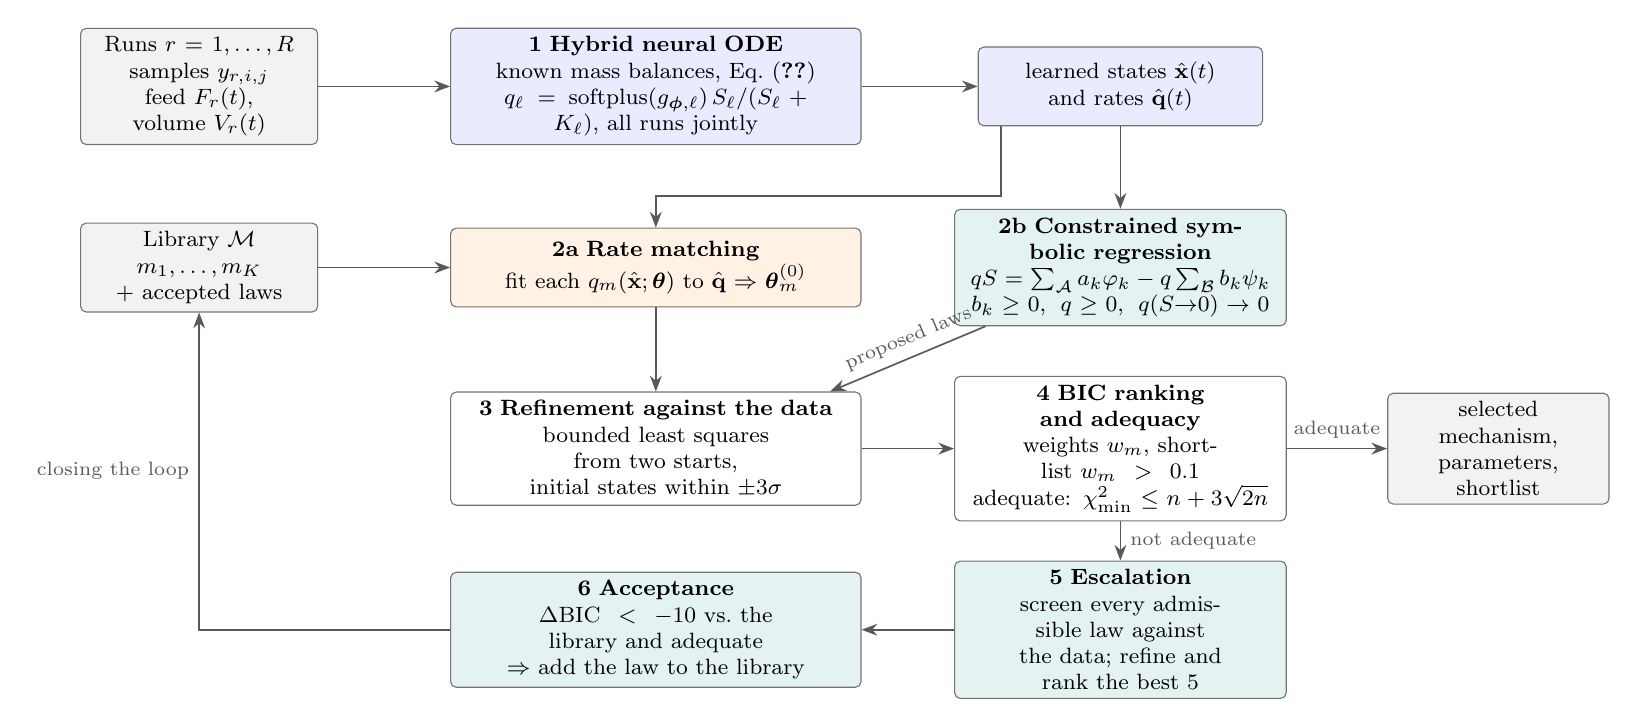
\begin{tikzpicture}[
  font=\footnotesize, >=Stealth,
  box/.style={draw=black!55, rounded corners=2pt, align=center, inner sep=3pt, minimum height=10mm, fill=white},
  datab/.style={box, fill=black!5},
  learnb/.style={box, fill=blue!8},
  mechb/.style={box, fill=orange!10},
  discb/.style={box, fill=teal!10},
  arr/.style={->, draw=black!65, line width=0.6pt},
  lab/.style={font=\scriptsize, text=black!65}]

% row 1: data and learning
\node[datab,  text width=28mm] (runs)  at (1.6, 0)   {Runs $r=1,\dots,R$\\ samples $y_{r,i,j}$\\ feed $F_r(t)$, volume $V_r(t)$};
\node[learnb, text width=50mm] (node)  at (7.4, 0)   {\textbf{1\;Hybrid neural ODE}\\ known mass balances, Eq.~\eqref{eq:massbalance}\\ $q_\ell=\mathrm{softplus}(g_{\boldsymbol\phi,\ell})\,S_\ell/(S_\ell+K_\ell)$, all runs jointly};
\node[learnb, text width=34mm] (rates) at (13.3, 0)  {learned states $\hat{\mathbf{x}}(t)$\\ and rates $\hat{\mathbf{q}}(t)$};

% row 2: candidates
\node[datab,  text width=28mm] (lib)   at (1.6, -2.3)  {Library $\mathcal{M}$\\ $m_1,\dots,m_K$\\ $+$ accepted laws};
\node[mechb,  text width=50mm] (match) at (7.4, -2.3)  {\textbf{2a\;Rate matching}\\ fit each $q_m(\hat{\mathbf{x}};\boldsymbol\theta)$ to $\hat{\mathbf{q}}$ $\Rightarrow$ $\boldsymbol\theta^{(0)}_m$};
\node[discb,  text width=40mm] (sr)    at (13.3, -2.3) {\textbf{2b\;Constrained symbolic regression}\\ $qS=\sum_{\mathcal{A}} a_k\varphi_k - q\sum_{\mathcal{B}} b_k\psi_k$\\ $b_k\ge0$,\; $q\ge0$,\; $q(S{\to}0)\to0$};

% row 3: refinement and ranking
\node[box,    text width=50mm] (ref)   at (7.4, -4.6)  {\textbf{3\;Refinement against the data}\\ bounded least squares from two starts,\\ initial states within $\pm3\sigma$};
\node[box,    text width=40mm] (sel)   at (13.3, -4.6) {\textbf{4\;BIC ranking and adequacy}\\ weights $w_m$, shortlist $w_m>0.1$\\ adequate: $\chi^2_{\min}\le n+3\sqrt{2n}$};
\node[datab,  text width=26mm] (res)   at (18.1, -4.6) {selected mechanism,\\ parameters,\\ shortlist};

% row 4: escalation and acceptance
\node[discb,  text width=40mm] (esc)   at (13.3, -6.9) {\textbf{5\;Escalation}\\ screen every admissible law against\\ the data; refine and rank the best 5};
\node[discb,  text width=50mm] (acc)   at (7.4, -6.9)  {\textbf{6\;Acceptance}\\ $\Delta\mathrm{BIC}<-10$ vs.\ the library and adequate\\ $\Rightarrow$ add the law to the library};

% arrows
\draw[arr] (runs) -- (node);
\draw[arr] (node) -- (rates);
\draw[arr] (rates) -- (sr);
\draw[arr] (rates.south west) ++(3mm,0) |- ($(match.north)+(0,4mm)$) -- (match.north);
\draw[arr] (lib) -- (match);
\draw[arr] (match) -- (ref);
\draw[arr] (sr.south west) ++(4mm,0) -- node[pos=0.45, above, sloped, lab] {proposed laws} ($(ref.north east)+(-4mm,0)$);
\draw[arr] (ref) -- (sel);
\draw[arr] (sel) -- node[above, lab] {adequate} (res);
\draw[arr] (sel) -- node[right, lab] {not adequate} (esc);
\draw[arr] (esc) -- (acc);
\draw[arr] (acc.west) -| node[pos=0.75, left, lab] {closing the loop} (lib.south);
\end{tikzpicture}}

\caption{Workflow. A hybrid neural ODE keeps the mass balances and learns the specific rates from one or several runs (step 1). The learned rates initialise every library mechanism (step 2a) and feed a physically constrained symbolic regression that proposes new rate laws (step 2b). All candidates are refined against the measurements and ranked by BIC (steps 3--4). If the best candidate does not fit within the measurement noise, every admissible law is screened against the data (step 5); a law that beats the library and fits within the noise is accepted and added to the library for later experiments (step 6).}
\label{fig:workflow}
\end{figure*}

\subsection{Problem formulation}\label{sec:m:problem}
An experiment consists of $R\ge 1$ fed-batch runs. In run $r$, offline samples are taken at times $t_{r,i}$ and give measurements $y_{r,i,j}$ of channels $j$ (biomass, substrates, products); not every channel is measured at every time, and $\Omega$ denotes the set of available measurements, $n=|\Omega|$. The feed rate $F_r(t)$, the feed composition $\mathbf{x}^{\mathrm{in}}_r$ and the culture volume $V_r(t)$ are recorded, so the dilution rate $D_r(t)=F_r(t)/V_r(t)$ is a known input. The concentrations $\mathbf{x}=(X,S_1,\dots,P,\dots)$ obey mass balances of the form
\begin{equation}
\frac{\dd \mathbf{x}}{\dd t} = \mathbf{N}(\boldsymbol{\eta})\,\mathbf{q}(\mathbf{x})\,X + D_r(t)\,\big(\mathbf{x}^{\mathrm{in}}_r - \mathbf{x}\big) - k_d X\,\mathbf{e}_X ,
\label{eq:massbalance}
\end{equation}
in which the stoichiometric matrix $\mathbf{N}$ contains the yields $\boldsymbol{\eta}$, $\mathbf{q}(\mathbf{x})$ is the vector of specific rates (growth, conversion), $k_d\ge 0$ is a first-order death rate and $\mathbf{e}_X$ selects the biomass equation. The structure of Eq.~\eqref{eq:massbalance} is known; the specific rates are not. A mechanism $m$ is a parametric rate law $\mathbf{q}_m(\mathbf{x};\boldsymbol{\theta}_m)$, and a library $\mathcal{M}$ collects the candidate mechanisms. The task is to decide which candidate (if any) governs the data, to estimate its parameters, and, when no candidate is adequate, to propose one that is.

\subsection{Step 1: hybrid neural ODE}\label{sec:m:node}
The specific rates are represented by a single multilayer perceptron $\mathbf{g}_{\boldsymbol{\phi}}$ (two hidden layers of 16 $\tanh$ units) that receives the concentrations on which the rates may depend, scaled by their largest measured values. Each rate $q_\ell$ is limited by a substrate $S_\ell$:
\begin{equation}
q_\ell(\mathbf{x}) = \softplus\!\big(g_{\boldsymbol{\phi},\ell}(\tilde{\mathbf{x}})\big)\,\frac{S_\ell}{S_\ell + K_\ell},
\label{eq:rate}
\end{equation}
with $\softplus(z)=\ln(1+e^{z})$.
The two factors encode the only assumptions that every candidate mechanism shares. The softplus keeps the rate non-negative (cell death is described separately by $k_d$), and the substrate factor makes the rate vanish smoothly when $S_\ell\to 0$, whatever the network outputs. The second constraint matters in fed-batch operation, where the culture spends most of the run substrate-limited: the substrate then settles at a low level $S^*_\ell$ at which uptake equals supply, which exists and is stable only if $q_\ell(S_\ell=0)=0$ and $q_\ell$ increases with $S_\ell$. Without the factor the network can assign a positive rate at zero substrate and the model consumes substrate that is not there (Section~\ref{sec:c1:node}). The constant $K_\ell$ is a fraction $\kappa_\ell$ of the typical substrate range, $K_\ell=\kappa_\ell\,\mathrm{median}_r\max_t S_{\ell,r}$, chosen close to the resolution of the data and large enough to keep the ODE non-stiff for an explicit integrator; it plays no role in the mechanisms that are eventually selected, whose parameters are estimated separately (Section~\ref{sec:m:refine}). The yields and $k_d$ are trainable scalars, kept positive through a logarithmic parameterisation.

The hybrid model is integrated with a fixed-step fourth-order Runge--Kutta scheme \citep{Chen2018}, all runs of an experiment at once as one batched state, and trained with Adam \citep{Kingma2015} on the range-scaled misfit
\begin{equation}
\mathcal{L}(\boldsymbol{\phi},\boldsymbol{\eta},k_d,\boldsymbol{\delta}) = \frac{1}{n}\sum_{(r,i,j)\in\Omega}\left(\frac{\hat{x}_{r,j}(t_{r,i}) - y_{r,i,j}}{s_{r,j}}\right)^2 ,
\label{eq:loss}
\end{equation}
where $s_{r,j}$ is the range of channel $j$ in run $r$. The initial state of each run is $\hat{\mathbf{x}}_r(0)=\mathbf{x}^0_r + 0.05\,\mathbf{s}\odot\boldsymbol{\delta}_r$, a trainable correction $\boldsymbol{\delta}_r$ to a data-based estimate $\mathbf{x}^0_r$: the intercept of a straight line through the samples taken within the first hour, or the first sample if only one is available, floored at 2\,\% of the channel maximum. Two details make training reliable. The fitting horizon grows from the first 25\,\% of the samples to all of them over the first half of the iterations, which avoids the spurious lag phases and stalls that appear when a full fed-batch trajectory is fitted from a random network; and the best full-horizon state is kept. Table~\ref{tab:settings} lists all settings.

\subsection{Step 2a: from learned rates to starting points}\label{sec:m:match}
The trained model provides dense trajectories $\hat{\mathbf{x}}(t)$ and rates $\hat{\mathbf{q}}(t)$ along every run. For each candidate $m$, its rate law is fitted to the learned rates,
\begin{equation}
\boldsymbol{\theta}^{(0)}_m = \arg\min_{\boldsymbol{\theta}} \sum_{\ell}\sum_{t\in\mathcal{T}} \left(\frac{q_{m,\ell}(\hat{\mathbf{x}}(t);\boldsymbol{\theta}) - \hat{q}_\ell(t)}{\max_t \hat{q}_\ell}\right)^2 ,
\label{eq:match}
\end{equation}
on a dense grid $\mathcal{T}$, with the yields and $k_d$ taken from the hybrid model; for the xylitol case the net growth rate $q_1-k_d$ is matched as well. This is an algebraic fit without ODE solves. It gives every candidate a starting point that reflects what the data say about the kinetics, rather than a generic point of its parameter box, at a cost that is negligible compared with the refinement.

\subsection{Step 2b: physically constrained symbolic regression}\label{sec:m:sr}
The library can only offer mechanisms that someone wrote down. To propose others, the learned rates are passed to a symbolic regression that searches over rate laws of the implicit form \citep{Mangan2016,Kaheman2020}
\begin{equation}
\begin{aligned}
q\,S &= \sum_{k\in\mathcal{A}} a_k\,\varphi_k(\mathbf{x}) - q\sum_{k\in\mathcal{B}} b_k\,\psi_k(\mathbf{x}),\\
\text{i.e.}\quad q &= \frac{\sum_{\mathcal{A}} a_k\varphi_k(\mathbf{x})}{S + \sum_{\mathcal{B}} b_k \psi_k(\mathbf{x})},
\end{aligned}
\label{eq:sr}
\end{equation}
where $S$ is the limiting substrate of the rate, $\{\varphi_k\}$ are numerator terms and $\{\psi_k\}$ denominator terms. For example, the Haldane law $\mu=\mu_{\max}S/(K_S+S+S^2/K_I)$ corresponds to $\mathcal{A}=\{S\}$ and $\mathcal{B}=\{1,S^2\}$. Exponential terms with a fitted constant, $S\,e^{-S/K}$ or $S\,e^{-P/K}$, extend the search to non-rational laws such as those of \citet{Teissier1942} and \citet{Aiba1968}. The dictionaries used in the case studies are listed in Sections~\ref{sec:case1} and \ref{sec:case2}.

The dictionaries are small, so every subset of terms up to a maximum size is evaluated (best-subset regression); sequentially thresholded least squares \citep{Brunton2016} approximates this search when the dictionary is too large to enumerate. Each subset defines a law whose coefficients are fitted to the learned rate \emph{in rate space}, by bounded nonlinear least squares on $q(\hat{\mathbf{x}}(t)) - \hat{q}(t)$, rather than by linear least squares on the implicit form of Eq.~\eqref{eq:sr}, which weights every sample by the square of the denominator and lets the high-substrate end of a run dominate. A law is kept only if it is physically admissible:
(i) it has at least one numerator term;
(ii) the denominator coefficients are non-negative, $b_k\ge 0$, so that the denominator is a sum of positive contributions as in every saturation or inhibition law (unconstrained fits readily produce denominators that change sign, i.e.\ rates that diverge);
(iii) every denominator term contributes along the trajectories;
(iv) the rate is non-negative along the trajectories; and
(v) the rate vanishes when the limiting substrate is exhausted, $q(S\to 0)\le 0.05\max_t\hat{q}$.
For each number of terms, the best admissible laws by rate-space error are retained. Each retained law---and, when the model has several rates, each combination of retained laws---becomes a candidate mechanism, with and without a death term. Its coefficients are bounded to $[0.1, 10]$ times their regression values with their signs preserved, and it is refined against the measurements (Section~\ref{sec:m:refine}) and ranked by BIC together with the library mechanisms. The regression therefore proposes; the measurements decide.

\subsection{Step 3: refinement against the measurements}\label{sec:m:refine}
Each candidate is then calibrated against the measurements by bounded nonlinear least squares,
\begin{equation}
\min_{\boldsymbol{\theta},\,\mathbf{x}_0}\ \chi^2_m = \sum_{(r,i,j)\in\Omega}\left(\frac{x_{r,j}(t_{r,i};\boldsymbol{\theta},\mathbf{x}_{0,r}) - y_{r,i,j}}{\sigma_{r,j}}\right)^2 ,
\label{eq:chi2}
\end{equation}
where the model is integrated with LSODA \citep{Petzold1983}. The kinetic parameters are bounded by $[0.1\,\boldsymbol{\ell}_m,\,5\,\mathbf{u}_m]$, generous multiples of physiological ranges $[\boldsymbol{\ell}_m,\mathbf{u}_m]$, and the initial states are estimated together with them within three noise standard deviations of $\mathbf{x}^0_r$: during exponential growth a small error in the initial biomass cannot be absorbed by any kinetic parameter. Because the parameters span several orders of magnitude, the optimisation is carried out in normalised coordinates $z = 1+(\theta-\theta^{\mathrm{lb}})/(\theta^{\mathrm{ub}}-\theta^{\mathrm{lb}})\in[1,2]$ with a trust-region reflective solver \citep{Branch1999} and forward-difference Jacobians with a relative step of $10^{-3}$. Every candidate is refined from two starting points, $\boldsymbol{\theta}^{(0)}_m$ and the centre of $[\boldsymbol{\ell}_m,\mathbf{u}_m]$, and the better fit is kept. Nested mechanisms provide a further check. A library mechanism that fits worse than a mechanism nested in it is usually trapped in a local minimum; it is then refined once more from the fit of the nested mechanism, with its additional terms made as weak as the bounds allow (inhibition constants at their upper bounds, death rate at its lower bound), for at most three rounds. In case study~2, whose mechanisms have up to nine parameters and four initial states per run, this restart was needed for the most complex mechanisms.

\subsection{Step 4: selection and adequacy}\label{sec:m:select}
With known measurement standard deviations $\sigma_{r,j}$ (the synthetic studies, where $\sigma_{r,j}$ is the noise level times the observed range of the channel) the candidates are ranked by Eq.~\eqref{eq:bic_bg}, where $k_m$ counts the kinetic parameters, yields and death rate; the initial states are common to all candidates and do not affect the ranking. The BIC weights $w_m$ are reported, and candidates with $w_m>0.1$ form a shortlist. The best candidate is \emph{adequate} if its residuals are compatible with the noise, which for a correct model gives $\chi^2\approx n-p$ with a standard deviation of about $\sqrt{2n}$; we use
\begin{equation}
\chi^2_{\min} \le n + 3\sqrt{2n}
\label{eq:adequacy}
\end{equation}
as the adequacy test.

For real data the error standard deviations are unknown. We assume one standard deviation $\sigma_j$ per measured species, shared across runs, and profile it out of the Gaussian likelihood \citep{BoxDraper1965,Bard1974}, which gives
\begin{equation}
\BIC_m = \sum_j n_j \ln\frac{\mathrm{RSS}_{m,j}}{n_j} + k_m \ln n ,
\label{eq:bic_profile}
\end{equation}
where $\mathrm{RSS}_{m,j}$ is the residual sum of squares of species $j$ and $n_j$ its number of measurements. The minimiser of Eq.~\eqref{eq:bic_profile} is obtained by iteratively reweighted least squares: Eq.~\eqref{eq:chi2} is solved with $\sigma_j$ fixed, $\sigma_j^2$ is re-estimated as $\mathrm{RSS}_{j}/n_j$, and the procedure is repeated three times. The bounds on the initial states are set once, with $\sigma_j$ equal to 5\,\% of the range of species $j$, so that a poor fit cannot widen them by inflating its own error estimate. Weighting by the estimated $\sigma_j$ also prevents the species with the largest concentrations (here, xylitol) from dominating the fit. The adequacy test is not available in this case.

\subsection{Steps 5--6: escalation and closing the loop}\label{sec:m:loop}
Ranking candidates by their match to the learned rates is a shortcut that works when the hybrid model is accurate. When the best library mechanism fails the adequacy test of Eq.~\eqref{eq:adequacy}, the shortcut is replaced by a screening of every admissible law (up to the maximum size) against the measurements: each law receives a short refinement of its coefficients and of the initial states (at most 50 objective evaluations), the laws are ranked by BIC, and the five best are refined fully, with and without a death term, and added to the ranking.

A proposed law is \emph{accepted} into the library when two conditions hold: it beats every library mechanism by $\Delta\BIC<-10$, which is very strong evidence on the usual scale \citep{Burnham2002}, and it passes the adequacy test. The second condition prevents a law that is merely better than the library, but still inconsistent with the data, from being carried into later analyses. An accepted law is stored with its terms and refined coefficients; in later experiments it is treated as any other mechanism, with a parameter box centred on the stored values and starting points from the stored values and from its terms refitted to the new learned rates.

\subsection{Implementation and evaluation protocol}\label{sec:m:impl}
The workflow is implemented in Python with PyTorch \citep{Paszke2019} and torchdiffeq \citep{Chen2018} for the hybrid model, SciPy \citep{Virtanen2020} for integration and least squares, and SymPy \citep{Meurer2017} to simplify the discovered laws. Each synthetic analysis runs on a single CPU core; for the real runs, the candidates of an analysis are refined in parallel. For the synthetic studies, measurements are generated by integrating the true model and adding Gaussian noise with a standard deviation equal to a fixed fraction of each channel's range, clipped at zero; every experiment is repeated for \ConeSeeds{} independent noise realisations, and the results are reported as frequencies and medians over the realisations.

\begin{table}[width=\linewidth,cols=3,pos=t]
\caption{Settings of the workflow. Where two values are given, the first applies to case study~1 and the second to case study~2.}\label{tab:settings}
\begin{tabular*}{\tblwidth}{@{}LL@{}}
\toprule
Item & Setting \\
\midrule
Rate network & MLP, 2 hidden layers $\times$ 16, $\tanh$ \\
Rate constraint & softplus $\times\, S/(S+K)$, Eq.~\eqref{eq:rate} \\
$\kappa$ in $K_\ell$ & 0.1; 0.25 (glucose), 0.1 (xylose) \\
Hybrid integrator & RK4, step 0.25\,h; 1\,h \\
Optimiser & Adam, learning rate $10^{-2}$ \\
Iterations & 300; 200 \\
Horizon curriculum & 25\,\% $\to$ 100\,\% of samples \\
Refinement solver & LSODA, rtol $10^{-6}$, atol $10^{-8}$ \\
Parameter bounds & $[0.1\,\boldsymbol{\ell},\,5\,\mathbf{u}]$ \\
Initial states & $\mathbf{x}^0 \pm 3\sigma$ (unknown $\sigma$: 5\,\% of range) \\
Starts & rate matching; range centre; \\
 & nested fit (case study 2) \\
Shortlist & $w_m > 0.1$ \\
Adequacy & $\chi^2_{\min}\le n+3\sqrt{2n}$ \\
SR terms (max.) & 4; 3 ($\mu_1$), 6 ($\mu_2$) \\
SR laws per size & 2; 1 \\
Escalation & all laws, $\le 50$ evaluations each; \\
 & best 5 refined fully \\
Acceptance & $\Delta\BIC<-10$ and adequate \\
\bottomrule
\end{tabular*}
\end{table}

\section{Case study 1: single-substrate fed-batch with a known ground truth}\label{sec:case1}

\subsection{System, library and experiments}\label{sec:c1:system}
The first case study is a single-substrate fed-batch culture with state $(X,S,V)$,
\begin{equation}
\begin{aligned}
\frac{\dd X}{\dd t} &= (\mu - k_d - D)X, \qquad \frac{\dd V}{\dd t} = F,\\
\frac{\dd S}{\dd t} &= -\frac{\mu X}{Y_{XS}} + D\,(S_{\mathrm{in}}-S),
\end{aligned}
\label{eq:c1}
\end{equation}
with $D=F/V$. The library contains eleven mechanisms (Table~\ref{tab:c1lib}): the Monod, Contois, Haldane and logistic biomass-inhibition laws, each with and without first-order death, and the Tessier, Moser and Aiba laws without death. The library is deliberately redundant. Monod, Tessier and Moser differ mainly at low substrate; Contois and Monod coincide when $K_cX\ll S$; Haldane and Aiba describe the same phenomenon, substrate inhibition, with rational and exponential forms; and a death term can be partly mimicked by a smaller yield. A twelfth, \emph{hidden} law combines Haldane substrate inhibition with logistic biomass inhibition,
\begin{equation}
\mu_{\mathrm{hidden}} = \mu_{\max}\frac{S}{K_S + S + S^2/K_I}\left(1-\frac{X}{X_{\max}}\right),
\label{eq:hidden}
\end{equation}
with $\mu_{\max}=0.6$\,h$^{-1}$, $K_S=1$\,g\,L$^{-1}$, $K_I=20$\,g\,L$^{-1}$ and $X_{\max}=30$\,g\,L$^{-1}$. Each of its ingredients is in the library, but their combination is not.

Every experiment consists of up to three 24\,h runs that differ in inoculum, initial substrate and feed (Fig.~\ref{fig:c1design}): run~a ($X_0=1$, $S_0=30$\,g\,L$^{-1}$) has a 6\,h batch phase followed by rising feed rates; run~b ($X_0=4$, $S_0=5$\,g\,L$^{-1}$) is fed from the start and stays substrate-limited at high biomass; and run~c ($X_0=0.5$, $S_0=60$\,g\,L$^{-1}$) keeps low biomass at high substrate. All runs start with $V_0=1.5$\,L and $S_{\mathrm{in}}=120$\,g\,L$^{-1}$ and are sampled 49 times, with Gaussian noise of 3\,\% of each channel's range on $X$ and $S$. Runs b and c place high biomass at low substrate and low biomass at high substrate in the same experiment, so that a rate that falls with $X$ and a rate that falls with $S$ predict different behaviour; in run~a alone, $X$ and $S$ move in opposite directions throughout (Fig.~\ref{fig:c1design}c). Each of the twelve generating laws (eleven library mechanisms and the hidden law) was simulated with the parameters of Table~\ref{tab:c1lib} for \ConeSeeds{} noise realisations. Every experiment was analysed twice, from run~a alone and from runs a--c jointly. The two analyses of an experiment took \ConeMinutes{}\,min together (median) on one CPU core.

\begin{table*}[width=\textwidth,cols=4,pos=t]
\caption{Case study 1: candidate mechanisms, parameter ranges $[\boldsymbol{\ell},\mathbf{u}]$ and true parameters of the generating models. Mechanisms marked $\pm k_d$ appear with and without death ($k_d\in[0.005,0.1]$\,h$^{-1}$, true value 0.04\,h$^{-1}$); $Y_{XS}\in[0.3,0.6]$ (true 0.5) for all. The hidden law of Eq.~\eqref{eq:hidden} is not in the library.}\label{tab:c1lib}
\begin{tabular*}{\tblwidth}{@{}LLLL@{}}
\toprule
Mechanism & $\mu(X,S)$ & Ranges & True parameters \\
\midrule
Monod $\pm k_d$ & $\mu_{\max}\,S/(K_S+S)$ & $\mu_{\max}\in[0.3,0.9]$, $K_S\in[0.1,5]$ & $\mu_{\max}=0.5$, $K_S=2$ \\
Contois $\pm k_d$ \citep{Contois1959} & $\mu_{\max}\,S/(K_cX+S)$ & $K_c\in[0.05,1]$ & $\mu_{\max}=0.5$, $K_c=1$ \\
Haldane $\pm k_d$ \citep{Andrews1968} & $\mu_{\max}\,S/(K_S+S+S^2/K_I)$ & $K_I\in[0.5,8]$ & $\mu_{\max}=0.6$, $K_S=1$, $K_I=8$ \\
Logistic $\pm k_d$ & $\mu_{\max}\,S/(K_S+S)\,(1-X/X_{\max})$ & $X_{\max}\in[12,40]$ & $\mu_{\max}=0.5$, $K_S=1$, $X_{\max}=20$ \\
Tessier \citep{Teissier1942} & $\mu_{\max}\,(1-e^{-S/K_S})$ & $K_S\in[0.1,5]$ & $\mu_{\max}=0.5$, $K_S=3$ \\
Moser \citep{Moser1958} & $\mu_{\max}\,S^{n}/(K_S+S^{n})$ & $K_S\in[0.1,25]$, $n\in[1,3]$ & $\mu_{\max}=0.5$, $K_S=16$, $n=2$ \\
Aiba \citep{Aiba1968} & $\mu_{\max}\,S/(K_S+S)\,e^{-S/K_I}$ & $K_I\in[5,50]$ & $\mu_{\max}=0.6$, $K_S=1$, $K_I=30$ \\
\bottomrule
\end{tabular*}
\end{table*}

\begin{figure*}
\centering
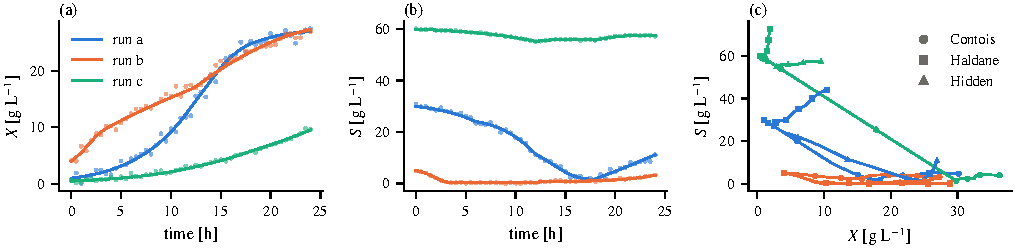
\includegraphics[width=\textwidth]{figs/c1_design.pdf}
\caption{Case study 1, experiment design (hidden law, first noise realisation). (a) Biomass and (b) substrate in the three runs; points are measurements, lines the noise-free trajectories. (c) The three runs in the $X$--$S$ plane for three generating laws: in run~a (blue) biomass and substrate move in opposite directions, whereas runs b and c reach high biomass at low substrate and low biomass at high substrate.}
\label{fig:c1design}
\end{figure*}

The symbolic-regression dictionary for $\mu$ contains the numerator terms $\{S,\ SX,\ S^2,\ S\,e^{-S/K}\}$ and the denominator terms $\{1,\ X,\ S^2,\ SX\}$, with laws of up to four terms. In the form of Eq.~\eqref{eq:sr}, Monod corresponds to $\{S;\,1\}$, Contois to $\{S;\,X\}$, Haldane to $\{S;\,1,S^2\}$, the logistic law to $\{S,SX;\,1\}$, Tessier to $\{S,\,S e^{-S/K}\}$, Aiba to $\{S e^{-S/K};\,1\}$, and the hidden law to $\{S,SX;\,1,S^2\}$. Moser, with a non-integer exponent, cannot be expressed.

\subsection{The hybrid model learns the kinetics}\label{sec:c1:node}
Figure~\ref{fig:c1mu} compares the specific growth rates learned by the hybrid model with the true ones along run~a. Without being told the mechanism, the network reproduces each law's signature: the abrupt drop of Monod, Tessier and Moser growth when the batch substrate is exhausted, the gradual decline of Contois and logistic growth as biomass accumulates, and the \emph{rise} of the Haldane and Aiba rates as an inhibitory substrate is consumed. The median training loss was \ConeNodeLossSingle{} on single runs, at the noise floor of $0.03^2\approx 9\times10^{-4}$ implied by Eq.~\eqref{eq:loss}, and \ConeNodeLossJoint{} on three runs, where one network must describe three regimes at once. The learned rates are therefore an accurate but not a perfect reference; the selection never relies on them alone.

\begin{figure*}
\centering
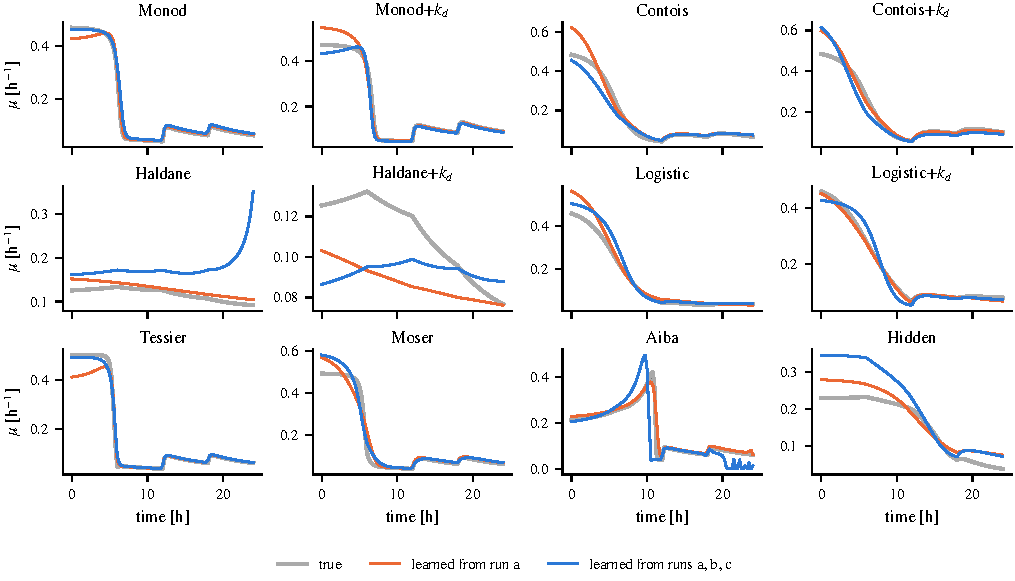
\includegraphics[width=\textwidth]{figs/c1_learned_mu.pdf}
\caption{Specific growth rate along run~a: true (grey) and learned by the hybrid neural ODE from run~a alone (orange) or from runs a--c jointly (blue), for the twelve generating laws (first noise realisation).}
\label{fig:c1mu}
\end{figure*}

The substrate factor in Eq.~\eqref{eq:rate} is essential when the culture becomes substrate-limited (Table~\ref{tab:ablation}). With a softplus output alone, the network assigns a positive growth rate at zero substrate; in the Monod experiment, which is substrate-limited for most of its duration, the model then drives the substrate below zero and the training loss and the error of the learned rate both increase several-fold. Runs whose substrate never falls near zero (Haldane) are unaffected.

\begin{table}[width=\linewidth,cols=7,pos=t]
\caption{Effect of the substrate factor $S/(S+K)$ in Eq.~\eqref{eq:rate}: medians over \ConeSeeds{} noise realisations of run~a. Loss in units of $10^{-3}$; rate error is the root-mean-square error of the learned $\mu$ relative to the maximum true $\mu$; $S_{\min}$ is the lowest substrate concentration of the trained model.}\label{tab:ablation}
\begin{tabular*}{\tblwidth}{@{}LCCCCCC@{}}
\toprule
 & \multicolumn{2}{c}{Loss} & \multicolumn{2}{c}{Rate error} & \multicolumn{2}{c}{$S_{\min}$ [g\,L$^{-1}$]} \\
Generating law & with & without & with & without & with & without \\
\midrule
\inputtab{generated/tab_c1_ablation.tex}
\bottomrule
\end{tabular*}
\end{table}

\subsection{Selection from one run is ambiguous}\label{sec:c1:single}
Table~\ref{tab:c1sel} and Fig.~\ref{fig:c1conf}a summarise the selection from run~a alone. With the four basic mechanisms as the library, the generating mechanism was selected in \ConeAccFour\,\% of the cases; with the full library of eleven, in \ConeAccSingle\,\%, with a mean BIC weight of \ConeWtrueSingle{} on the true mechanism and the true mechanism on the shortlist in \ConeShortSingle\,\%. Every best fit passed the adequacy test, so the errors are not failures of the fitting but ambiguities of the data. They follow the structure of the library. Monod, Tessier, Moser and Contois share the weight, because they differ mainly in the brief low-substrate window that a fed-batch run crosses quickly. Haldane is read as Contois or Aiba: along run~a the substrate falls while biomass rises, so a growth rate that changes because $S$ falls cannot be told apart from one that changes because $X$ rises. Aiba and Haldane+$k_d$ are confused with each other, as two forms of substrate inhibition. Death variants are partly confused with their death-free counterparts.

\begin{table}[width=\linewidth,cols=6,pos=t]
\caption{Case study 1: selection accuracy [\%] and mean BIC weight of the generating mechanism over \ConeSeeds{} noise realisations, from run~a alone with the four-mechanism and the eleven-mechanism library, and from runs a--c jointly with the eleven-mechanism library.}\label{tab:c1sel}
\tabcolsep=3.5pt
\begin{tabular*}{\tblwidth}{@{}LCCCCC@{}}
\toprule
 & 4 mech. & \multicolumn{2}{c}{11 mech., run a} & \multicolumn{2}{c}{11 mech., runs a--c} \\
Generating law & acc. & acc. & weight & acc. & weight \\
\midrule
\inputtab{generated/tab_c1_selection.tex}
\bottomrule
\end{tabular*}
\end{table}

\subsection{Three jointly fitted runs resolve the ambiguity}\label{sec:c1:joint}
Fitting runs a--c jointly, with shared kinetic parameters and one initial state per run, removes the ambiguity (Fig.~\ref{fig:c1conf}b): the generating mechanism was selected in \ConeAccJoint\,\% of the \ConeLibCasesJoint{} library cases, with a mean weight of \ConeWtrueJoint{}. The remaining weight sits on nested alternatives with one extra parameter (a death term, or the Moser exponent). The two additional runs do not add new kinds of measurements; they add operating points at which the candidates make different predictions. Haldane, for example, is identified because run~c keeps the substrate in the inhibitory range at low biomass, where a Contois or logistic law predicts fast growth.

\begin{figure*}
\centering
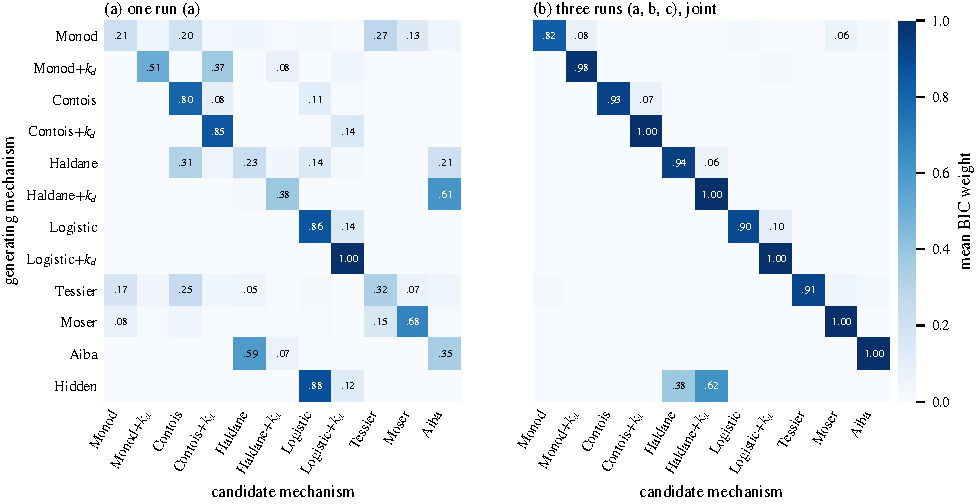
\includegraphics[width=\textwidth]{figs/c1_confusion.pdf}
\caption{Case study 1: mean BIC weight of every candidate (columns) for every generating law (rows) over \ConeSeeds{} noise realisations, (a) from run~a alone and (b) from runs a--c jointly. The last row is the hidden law, which is not in the library.}
\label{fig:c1conf}
\end{figure*}

\subsection{Symbolic regression: no false discoveries, non-rational laws recovered}\label{sec:c1:sr}
Symbolic regression proposed seven laws per analysis, which were refined with and without a death term and ranked together with the library. Figure~\ref{fig:c1sr} shows, for every analysis, the BIC difference between the best proposed law and the best library mechanism. For the eleven library experiments the proposed laws never met the acceptance rule (\ConeFalseDiscSingle{} of \ConeLibCasesSingle{} single-run and \ConeFalseDiscJoint{} of \ConeLibCasesJoint{} joint analyses): when the generating law is in the library, the regression does not produce spurious discoveries. In many of these cases the best proposed law \emph{is} the library law written in the form of Eq.~\eqref{eq:sr} and ties with it ($\Delta\BIC\approx 0$; Table~\ref{tab:c1sr}). This includes the two non-rational laws: the exponential dictionary term recovered the Aiba structure in \ConeAibaRedisc\,\% and the Tessier structure in \ConeTessierRedisc\,\% of the joint analyses. Moser, which the dictionary cannot express, was always better described by its library entry ($\Delta\BIC\approx 95$).

\begin{table}[width=\linewidth,cols=3,pos=t]
\caption{Case study 1, symbolic regression on runs a--c jointly: frequency [\%] with which the generating structure was among the proposed laws within two BIC units of the best one, and median BIC difference between the best proposed law and the best library mechanism (positive: the library mechanism is preferred).}\label{tab:c1sr}
\begin{tabular*}{\tblwidth}{@{}LCC@{}}
\toprule
Generating law & Structure recovered & Median $\Delta\BIC$ \\
\midrule
\inputtab{generated/tab_c1_sr.tex}
\bottomrule
\end{tabular*}
\end{table}

\begin{figure*}
\centering
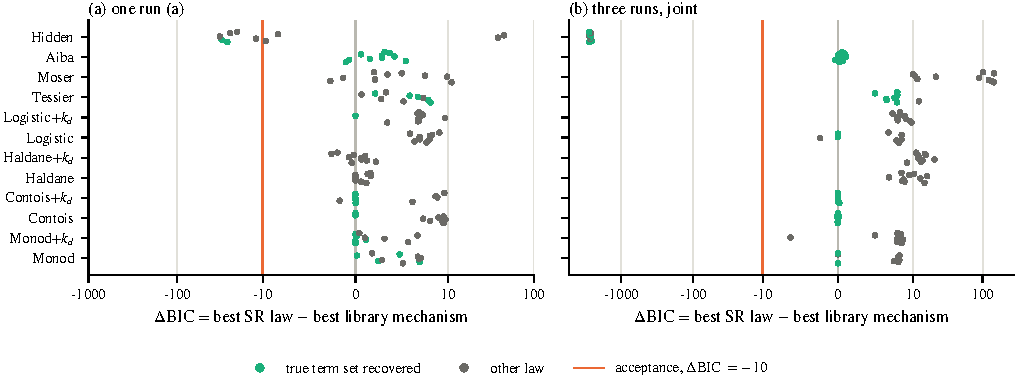
\includegraphics[width=\textwidth]{figs/c1_sr.pdf}
\caption{Case study 1: BIC difference between the best law proposed by symbolic regression and the best library mechanism, for every generating law and noise realisation, (a) from run~a alone and (b) from runs a--c jointly (symmetric logarithmic axis). Green: the generating structure is among the proposed laws within two BIC units of the best one. The orange line marks the acceptance threshold $\Delta\BIC=-10$; only the hidden law crosses it.}
\label{fig:c1sr}
\end{figure*}

\subsection{A mechanism missing from the library}\label{sec:c1:hidden}
For the hidden law the behaviour depends on the data. From run~a alone the best library mechanism, the logistic law, fits within the noise (median $\chi^2=\ConeHiddenChiLibSingle$ against the adequacy limit of \ConeChiOKsingle{} for $n=98$), so nothing indicates that the library is incomplete. Symbolic regression nevertheless proposed a better law in \ConeHiddenBestSingle{} of \ConeHiddenN{} realisations and one that met the acceptance rule in \ConeHiddenAcceptedSingle{}, but the proposed structure was the true one in only \ConeHiddenFoundSingle{}. A single run thus contains evidence that the library is missing something, but not enough to say what.

With three runs the picture changes (Fig.~\ref{fig:c1hidden}). The best library mechanism, now Haldane, fails the adequacy test in \ConeHiddenFlagJoint{} of \ConeHiddenN{} realisations (median $\chi^2=\ConeHiddenChiLib$ against a limit of \ConeChiOK{} for $n=294$), which triggers the escalation: all \ConeScreened{} admissible laws are screened against the measurements and the five best are refined. The best law then fits within the noise (median $\chi^2=\ConeHiddenChiSR$) and is accepted in \ConeHiddenAcceptedJoint{} of \ConeHiddenN{} realisations. Its structure is exactly that of the hidden law, $\{S,SX;\,1,S^2\}$, in \ConeHiddenFoundJoint{} realisations; in the other \ConeHiddenEquivJoint{}, the numerator term $S$ is replaced by $S\,e^{-S/K}$ with $K$ between \ConeHiddenKmin{} and \ConeHiddenKmax{}\,g\,L$^{-1}$, a factor between 0.86 and 1 over the observed substrate range, i.e.\ the same law for all practical purposes. For the first realisation the discovered law, rewritten in the conventional form, is
\begin{equation}
\mu = \ConeHidMumax\,\frac{S\,\big(1 - X/\ConeHidXmax\big)}{\ConeHidKs + S + S^2/\ConeHidKi},
\label{eq:discovered}
\end{equation}
against the true $\mu_{\max}=0.6$\,h$^{-1}$, $X_{\max}=30$, $K_S=1$ and $K_I=20$\,g\,L$^{-1}$.

The escalation was necessary. The true structure was never among the laws shortlisted by their match to the learned rates (\ConeHiddenShortTrue{} of \ConeHiddenN{} realisations), and the best shortlisted law passed the adequacy test in only \ConeHiddenPreOK{}. The reason is the accuracy of the learned rate: along run~a it deviated from the true rate by up to \ConeHiddenErrAmax\,\% of its maximum (median \ConeHiddenErrAmed\,\%), against at most \ConeHiddenErrBCmax\,\% along runs b and c. With errors of this size, a wrong law can match the learned rate better than the true one. The screening against the measurements does not depend on the learned rates and corrects this.

\begin{figure*}
\centering
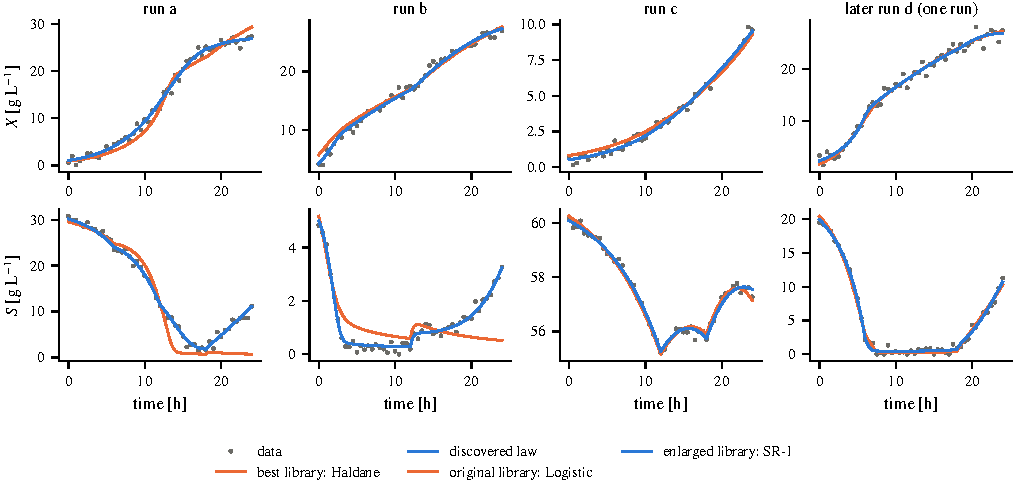
\includegraphics[width=\textwidth]{figs/c1_hidden.pdf}
\caption{Hidden law (first noise realisation). Runs a--c: measurements, best library mechanism (Haldane, orange) and the law discovered after escalation (blue), all fitted jointly. Later run d: a single new run analysed with the original library (orange; best: logistic) and with the library enlarged by the discovered law (blue).}
\label{fig:c1hidden}
\end{figure*}

\paragraph{Closing the loop}
The accepted law was added to the library (as ``SR-1'') and the enlarged library was used, without symbolic regression, on a later single run under new conditions (run~d: $X_0=2$, $S_0=20$\,g\,L$^{-1}$, $S_{\mathrm{in}}=150$\,g\,L$^{-1}$, a different feed). With the original library the logistic law was selected in \ConeLaterBaseCount{} of \ConeLoopN{} realisations. With the enlarged library, SR-1 fitted run~d better than every original mechanism in \ConeLaterBetterChi{} realisations (by up to \ConeLaterDchiMax{} $\chi^2$ units) and was selected with a weight above 0.9 in \ConeLaterStrong{}; in the others the logistic law, with one parameter fewer, was preferred. Run~d never exceeds about 20\,g\,L$^{-1}$ of substrate, where the inhibition term of the hidden law is weak, so a single run in this regime gives only moderate evidence for it; the library entry nevertheless makes the better law available. Conversely, refined on the eleven library experiments, SR-1 never took more than \ConeStealMax{} of the BIC weight and did not change any selection (\ConeStealChanged{} of \ConeStealCases{}): enlarging the library did not compromise the identification of the existing mechanisms.

\section{Case study 2: xylitol bioconversion in fed-batch culture}\label{sec:case2}

\subsection{Process, data and model}\label{sec:c2:system}
The second case study concerns the bioconversion of xylose into xylitol by \emph{Saccharomyces cerevisiae} H1274, a strain that expresses the xylose reductase of \emph{Pichia stipitis} from a multicopy plasmid \citep{Toivari2025,ToivariData2025}. The strain does not grow on xylose; it reduces xylose to xylitol with NADPH that is regenerated by the metabolism of glucose, which is therefore supplied as a co-substrate. Four fed-batch cultures in yeast extract--peptone medium, labelled BC12, BC15, BC18 and BC19, are analysed. Each starts with a batch phase on about 20\,g\,L$^{-1}$ glucose, during which ethanol accumulates and is subsequently consumed, and continues with a feed of glucose and xylose (83--109 and 260--334\,g\,L$^{-1}$, respectively) at about 1.5--2\,mL\,h$^{-1}$ for 98--171\,h, while the culture volume grows from 0.27--0.30\,L to 0.40--0.48\,L. The runs differ in ways that matter for kinetics: in BC12 the batch medium already contains 63\,g\,L$^{-1}$ xylose and the feed starts only after 24\,h, whereas BC15, BC18 and BC19 start without xylose and are fed from about 8\,h; BC19 was supplemented with corn steep solids. Biomass (dry weight), glucose, ethanol, xylose and xylitol were measured at 8--11 times per run.

The state is $(X,S_1,S_2,P)$: biomass, glucose equivalent, xylose and xylitol. Glucose and the ethanol produced from it during the batch phase are lumped into one growth substrate, $S_1=\text{glucose}+1.2\,\text{ethanol}$ (in g\,L$^{-1}$), in both the culture and the feed. With the dilution rate $D(t)=F(t)/V(t)$ computed from the recorded feed rate and the measured volume, the mass balances are
\begin{equation}
\begin{aligned}
\frac{\dd X}{\dd t} &= (\mu_1 - k_d - D)\,X, \\
\frac{\dd S_1}{\dd t} &= -\frac{\mu_1 X}{Y_{XS_1}} + D\,(S_{1}^{\mathrm{in}} - S_1),\\
\frac{\dd S_2}{\dd t} &= -\frac{\mu_2 X}{Y_{PS_2}} + D\,(S_{2}^{\mathrm{in}} - S_2),\\
\frac{\dd P}{\dd t} &= \mu_2 X - D\,P,
\end{aligned}
\label{eq:c2}
\end{equation}
where $\mu_1$ is the specific growth rate on the glucose equivalent, $\mu_2$ the specific rate of xylitol formation, $Y_{XS_1}$ the biomass yield on the glucose equivalent and $Y_{PS_2}$ the xylitol yield on xylose. The library (Table~\ref{tab:c2lib}) contains eleven mechanisms built from a Monod baseline for both rates by adding inhibition of growth by xylitol ($K_{PI_1}$) or by xylose ($K_{SI_1}$), substrate inhibition of the conversion ($K_{SI_2}$), product inhibition of the conversion ($K_{PI_2}$), and first-order death:
\begin{equation}
\begin{aligned}
\mu_1 &= \frac{\mu_{\max,1}\,S_1}{K_{S_1}+S_1+S_2^2/K_{SI_1}}\cdot\frac{1}{1+P/K_{PI_1}},\\
\mu_2 &= \frac{\mu_{\max,2}\,S_2}{K_{S_2}+S_2+S_2^2/K_{SI_2}}\cdot\frac{1}{1+P/K_{PI_2}},
\end{aligned}
\label{eq:c2lib}
\end{equation}
where a term or factor is absent when its constant does not appear in the mechanism. Mechanisms M22--M27 modify the growth rate and M28--M31 the conversion rate; M31, the most complex, combines both conversion inhibitions with death.

\begin{table*}[width=\textwidth,cols=4,pos=t]
\caption{Case study 2: library mechanisms (Eq.~\eqref{eq:c2lib}) and parameter ranges $[\boldsymbol{\ell},\mathbf{u}]$. All mechanisms contain $\mu_{\max,1}\in[0.05,0.8]$\,h$^{-1}$, $K_{S_1}\in[0.05,0.2]$\,g\,L$^{-1}$, $K_{S_2}\in[40,120]$\,g\,L$^{-1}$, $Y_{XS_1}\in[0.1,1.2]$ and $Y_{PS_2}\in[0.5,2]$\,g\,g$^{-1}$; $\mu_{\max,2}\in[1,6]$\,h$^{-1}$ for M21--M27 and $[1,8]$\,h$^{-1}$ for M28--M31. Refinement bounds are $[0.1\,\boldsymbol{\ell},\,5\,\mathbf{u}]$.}\label{tab:c2lib}
\begin{tabular*}{\tblwidth}{@{}LLLL@{}}
\toprule
Mechanism & Additional terms & Ranges of the additional parameters & $k$ \\
\midrule
M21 & -- (Monod for $\mu_1$ and $\mu_2$) & -- & 6 \\
M22 & xylitol inhibits growth & $K_{PI_1}\in[10,50]$ & 7 \\
M23 & xylose inhibits growth & $K_{SI_1}\in[20,100]$ & 7 \\
M24 & xylose and xylitol inhibit growth & $K_{SI_1}$, $K_{PI_1}$ & 8 \\
M25 & death; xylitol inhibits growth & $k_d\in[0.005,0.1]$\,h$^{-1}$, $K_{PI_1}$ & 8 \\
M26 & death; xylose inhibits growth & $k_d$, $K_{SI_1}$ & 8 \\
M27 & death; xylose and xylitol inhibit growth & $k_d$, $K_{SI_1}$, $K_{PI_1}$ & 9 \\
M28 & xylitol inhibits conversion & $K_{PI_2}\in[2,20]$ & 7 \\
M29 & xylose inhibits conversion (Haldane) & $K_{SI_2}\in[2,50]$ & 7 \\
M30 & xylose and xylitol inhibit conversion & $K_{SI_2}$, $K_{PI_2}$ & 8 \\
M31 & death; xylose and xylitol inhibit conversion & $k_d$, $K_{SI_2}$, $K_{PI_2}\in[2,50]$ & 9 \\
\bottomrule
\end{tabular*}
\end{table*}

The hybrid model replaces $\mu_1$ and $\mu_2$ by the two outputs of one network with inputs $(S_1,S_2,P)$, limited by $S_1$ and $S_2$, respectively (Eq.~\eqref{eq:rate}); $Y_{XS_1}$, $Y_{PS_2}$ and $k_d$ are trained with the network. The symbolic-regression dictionaries are, for $\mu_1$ with limiting substrate $S_1$, the numerator term $\{S_1\}$ and the denominator terms $\{1,\ S_2^2,\ P,\ S_1P\}$ (laws of up to three terms), and, for $\mu_2$ with limiting substrate $S_2$, the numerator terms $\{S_2,\ S_2\,e^{-P/K}\}$ and the denominator terms $\{1,\ S_2^2,\ P,\ S_2P,\ S_2^2P\}$ (up to six terms). They contain the conversion laws of the library---M28 is $\{S_2;\,1,P,S_2P\}$, M29 $\{S_2;\,1,S_2^2\}$ and M30 $\{S_2;\,1,S_2^2,P,S_2P,S_2^2P\}$---and, through the exponential term, exponential product inhibition $\mu_2 = a\,S_2\,e^{-P/K}/(b+S_2)$, the form proposed by \citet{Aiba1968} for ethanol fermentation. The growth dictionary is deliberately smaller: growth occurs mainly in the short batch phase, which is covered by two or three samples. The best law of each size is retained for each rate, and every combination of a $\mu_1$ and a $\mu_2$ law, with and without death, becomes a candidate (at most 36 per analysis).

\subsection{Virtual runs with the sampling of real experiments}\label{sec:c2:virtual}
Before the real data, the workflow was tested on virtual runs that keep everything of a real run except the kinetics: its feed profile, volume, initial state and sampling schedule, including missing values. Run V18 reproduces BC18 with kinetics M31, and run V15 reproduces BC15 with M28, each with the parameters obtained by calibrating that mechanism to the corresponding real run (Section~\ref{sec:c2:real}; Table~\ref{tab:c2virtualpar} in Appendix~\ref{app:c2}), and with Gaussian noise of 5\,\% of each channel's range; \VeighteenN{} noise realisations of each were analysed with the measurement noise known. The virtual runs carry the information content of a real experiment---eight to ten samples per species, three of them in the batch phase---rather than the dense sampling of case study~1.

\begin{table*}[width=\textwidth,cols=8,pos=t]
\caption{Case study 2, virtual runs: selection over \VeighteenN{} noise realisations. Accuracy and shortlist frequency in \%, mean BIC weight of the generating mechanism, wrong selections (with counts), median BIC difference between the best symbolic-regression law and the best library mechanism, and number of accepted discoveries.}\label{tab:c2virtual}
\begin{tabular*}{\tblwidth}{@{}LLCCCLCC@{}}
\toprule
Run & True & Accuracy & Weight & Shortlist & Other selections & Median $\Delta\BIC_{\mathrm{SR}}$ & Accepted \\
\midrule
\inputtab{generated/tab_c2_virtual.tex}
\bottomrule
\end{tabular*}
\end{table*}

The hybrid model reproduced the virtual measurements to a median loss of \VeighteenNodeLoss{} (V18) and \VfifteenNodeLoss{} (V15), and its learned rates follow the true ones (Fig.~\ref{fig:c2virtual}): the drop of $\mu_1$ when the batch glucose is exhausted, the peak of $\mu_2$ when xylose first appears and its slow decline as xylitol accumulates. The learned rates are least accurate in V15, where $\mu_1$ is overestimated in the batch phase and the peak of $\mu_2$ is smoothed out; the subsequent refinement against the measurements does not inherit these errors. Table~\ref{tab:c2virtual} gives the selection results. M31 was identified in all V18 realisations with a mean weight of \VeighteenW{}: BC18-type data require both death, which explains the slowly falling biomass, and inhibition of the conversion, which explains the slowing xylitol production, and only M31 has both. V15 is harder. M28 was selected in \VfifteenAcc\,\% of the realisations and was always shortlisted, but with a mean weight of only \VfifteenW{}; most of the remaining weight went to \VfifteenAlts. In a BC15-type run xylose and xylitol both increase monotonically during the feed, so a conversion rate that declines because xylitol accumulates (M28) and one that declines because xylose accumulates (M29) are hard to separate---the same confounding of two monotone trends that made single runs ambiguous in case study~1.

\begin{figure*}
\centering
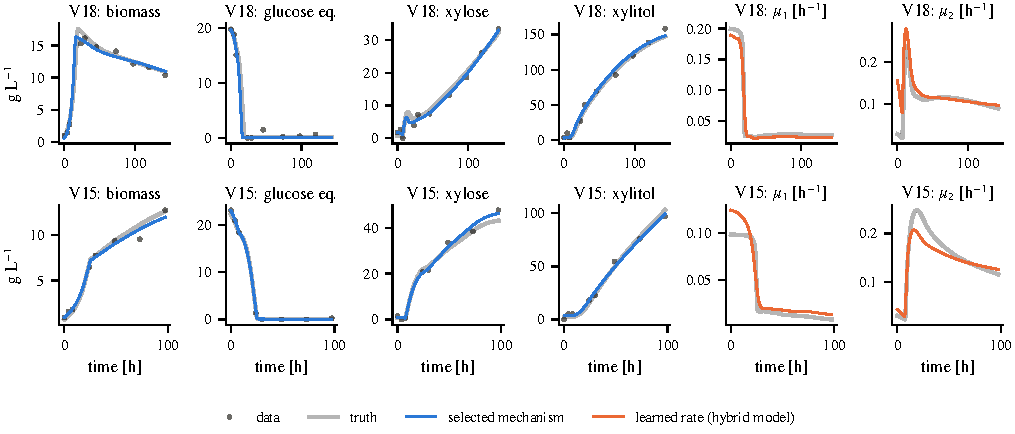
\includegraphics[width=\textwidth]{figs/c2_virtual.pdf}
\caption{Case study 2, virtual runs V18 (top, true mechanism M31) and V15 (bottom, true mechanism M28), first noise realisation: measurements, true trajectories and the trajectories of the selected mechanism, and the specific rates $\mu_1$ and $\mu_2$ learned by the hybrid model compared with the true ones.}
\label{fig:c2virtual}
\end{figure*}

Symbolic regression produced no false discoveries (\VeighteenFD{} and \VfifteenFD{} accepted laws). In \VirtSRexp{} of the \VirtSRn{} analyses, the best proposed conversion law contained the exponential product-inhibition term, and in \VirtSRexpMonod{} it was exactly $\mu_2=a\,S_2\,e^{-P/K}/(b+S_2)$, which reproduces the hyperbolic product inhibition of M28 and M31 within the noise over the observed range of $P$. On V18 it ranks marginally ahead of M31 (median $\Delta\BIC=\VeighteendBICmed$, never below \VeighteendBICmin), because it describes the same behaviour with one parameter fewer; on V15 it ties with M28 (median \VfifteendBICmed). The best proposed law included a death term where the generating mechanism has one and omitted it where it does not in \VirtSRdeath{} of the \VirtSRn{} analyses. Both are far from the acceptance threshold: an alternative functional form of the same mechanism is proposed, compared and correctly not accepted.

\subsection{Real runs analysed individually}\label{sec:c2:real}
For the real runs the measurement errors are unknown, and the candidates were ranked by the profile-likelihood criterion of Eq.~\eqref{eq:bic_profile} with one error standard deviation per species. Table~\ref{tab:c2real} and Fig.~\ref{fig:c2weights} summarise the selection and Fig.~\ref{fig:c2real} shows the fits. Each run was analysed in \BCfifteenMinutes--\BCtwelveMinutes\,min, with the candidates refined in parallel.

\begin{table*}[width=\textwidth,cols=9,pos=t]
\caption{Case study 2, real runs: number of measurements, selected mechanism and shortlist (BIC weights in parentheses), residual standard deviations of the selected mechanism [g\,L$^{-1}$], and BIC difference between the best symbolic-regression law and the selected mechanism (negative: the proposed law is preferred).}\label{tab:c2real}
\begin{tabular*}{\tblwidth}{@{}LCLLCCCCC@{}}
\toprule
Analysis & $n$ & Selected & Shortlist & $X$ & $S_1$ & $S_2$ & $P$ & $\Delta\BIC_{\mathrm{SR}}$ \\
\midrule
\inputtab{generated/tab_c2_real.tex}
\bottomrule
\end{tabular*}
\end{table*}

\begin{figure}
\centering
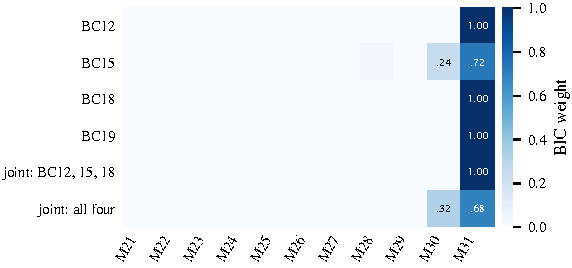
\includegraphics[width=\linewidth]{figs/c2_real_weights.pdf}
\caption{Case study 2, real runs: BIC weights of the eleven library mechanisms for each run analysed alone and for the joint analyses.}
\label{fig:c2weights}
\end{figure}

\begin{figure*}
\centering
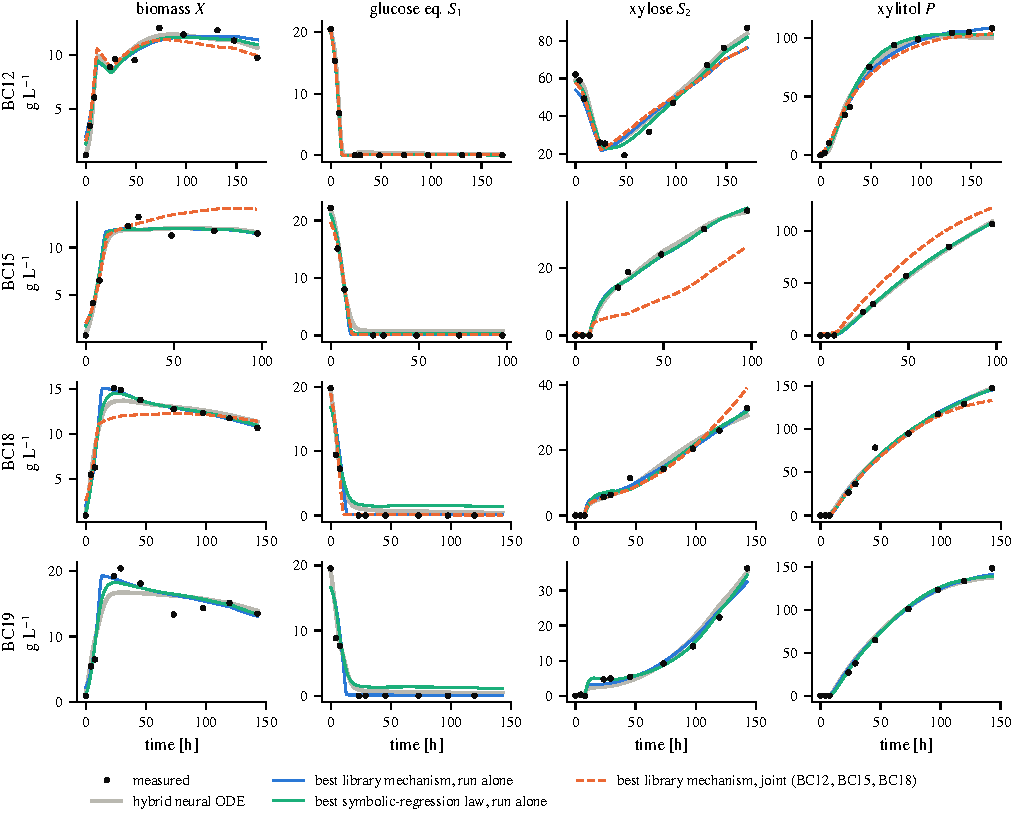
\includegraphics[width=\textwidth]{figs/c2_real.pdf}
\caption{Case study 2, real runs BC12, BC15, BC18 and BC19 (rows): measurements, hybrid neural ODE, best library mechanism and best symbolic-regression law fitted to each run alone, and best library mechanism fitted to BC12, BC15 and BC18 jointly.}
\label{fig:c2real}
\end{figure*}

M31 was selected for every run, with a weight of \BCtwelveW{} for BC12, \BCeighteenW{} for BC18 and \BCnineteenW{} for BC19, and \BCfifteenW{} for BC15, where M30, the same mechanism without death, took most of the remaining weight. The four runs therefore agree on the qualitative mechanism: xylitol formation slows down because both xylose and xylitol inhibit it, and the biomass declines through first-order death during the long production phase. It is consistent with the hybrid model, which learned death rates of 0.013--0.020\,h$^{-1}$ and a conversion rate that declines during the feed phase in BC12, BC18 and BC19 and stays nearly constant in BC15. The residual standard deviations are 1--10\,\% of the ranges of the measured species, with two systematic deviations visible in Fig.~\ref{fig:c2real}. First, the fitted initial biomass exceeds the first measurement by \BCtwelveDXzero, \BCfifteenDXzero, \BCeighteenDXzero{} and \BCnineteenDXzero\,g\,L$^{-1}$ in the four runs, close to the bound of the initial states. This is a limitation shared by all candidates: with a single growth substrate, the model cannot represent the batch phase, in which the yeast grows fast on glucose and then more slowly on the ethanol it produced, and it compensates through the initial biomass. Second, in BC12, the only run with xylose in the batch medium, M31 misses the minimum of the xylose concentration by up to 11\,g\,L$^{-1}$.

The parameter values differ between the runs (Table~\ref{tab:c2params}), and several are poorly determined. The constants of the conversion rate trade off against each other: $K_{S_2}$ lies far above the observed xylose concentrations in three runs, while $K_{SI_2}$ varies between 0.3 and 13\,g\,L$^{-1}$; and $K_{S_1}$ reached its upper bound in two runs. The rates implied by the fits are more comparable than the constants: evaluated at a common state ($S_2=30$ and $P=50$\,g\,L$^{-1}$), the conversion rate of the selected mechanism is \BCtwelveMuRef, \BCfifteenMuRef{} and \BCeighteenMuRef\,h$^{-1}$ for BC12, BC15 and BC18, but only \BCnineteenMuRef\,h$^{-1}$ for BC19, the run supplemented with corn steep solids.

\begin{table*}[width=\textwidth,cols=7,pos=t]
\caption{Case study 2: parameters of M31 fitted to each real run alone and to groups of runs jointly with shared parameters.}\label{tab:c2params}
\begin{tabular*}{\tblwidth}{@{}LCCCCCC@{}}
\toprule
Parameter & \inputtab{generated/tab_c2_real_params_head.tex} \\
\midrule
\inputtab{generated/tab_c2_real_params.tex}
\bottomrule
\end{tabular*}
\end{table*}

\subsection{Real runs analysed jointly}\label{sec:c2:joint}
In case study~1, fitting several runs jointly resolved the ambiguity of single runs. That required the runs to share their kinetics, which held by construction. For real runs it is a hypothesis, and it can be tested with the same criterion: the BIC of a joint fit with one set of kinetic parameters is compared with the BIC of separate fits of the same runs, both evaluated with one error standard deviation per species pooled over the runs (Table~\ref{tab:c2shared}). Because the separate fits were obtained with run-specific error weights, their pooled criterion is an upper bound on its optimum, and the comparison is conservative with respect to separate kinetics.

\begin{table}[width=\linewidth,cols=5,pos=t]
\caption{Case study 2: shared versus run-specific kinetics. BIC of M31 fitted jointly with shared parameters minus BIC of M31 fitted to each run separately, both with one error standard deviation per species pooled over the runs (positive: run-specific parameters are preferred); $k$ counts the kinetic parameters.}\label{tab:c2shared}
\begin{tabular*}{\tblwidth}{@{}LCCCC@{}}
\toprule
Runs & $n$ & $k$ shared & $k$ separate & $\Delta\BIC$ \\
\midrule
\inputtab{generated/tab_c2_shared.tex}
\bottomrule
\end{tabular*}
\end{table}

Joint fitting again selected M31: with a weight of \JointThreeW{} for the three runs in yeast extract--peptone medium (BC12, BC15 and BC18) and of \JointFourW{} for all four runs, with M30 taking the rest (Table~\ref{tab:c2real}, Fig.~\ref{fig:c2weights}). The shared parameters, however, do not describe the runs equally well. In the joint fit of BC12, BC15 and BC18, the residual standard deviations of xylose and xylitol in BC15 rise from about 1\,g\,L$^{-1}$ in its individual fit to 9 and 12\,g\,L$^{-1}$ (Fig.~\ref{fig:c2real}, dashed lines), and the fitted initial biomass of the four-run fit lies 1.8--2.9\,g\,L$^{-1}$ above the first measurements, at the bounds of the initial states. Accordingly, run-specific parameters were preferred for every group of runs tested (Table~\ref{tab:c2shared}), with $\Delta\BIC=\SharedThree$ for the three runs in the same medium and $\Delta\BIC=\SharedTwo$ for BC15 and BC18, the two runs with the most similar operation. The real runs therefore share a mechanism but not its parameter values, and the differences are larger than their measurement errors.

This has a direct consequence for the symbolic regression. For the joint analyses the best proposed laws were preferred to M31 beyond the acceptance threshold ($\Delta\BIC=\JointThreeSRdBIC$ and $\JointFourSRdBIC$; Table~\ref{tab:c2sr}). Both have the same structure, a Monod-type conversion rate with an additional numerator term that decays exponentially with xylitol and a combined inhibition term $PS_2^2$ in the denominator, and their additional terms may absorb part of the differences between the runs: in the three-run fit, for instance, the exponential term has fallen to 10\,\% at 3\,g\,L$^{-1}$ xylitol and only describes a transient at the start of the feed. A law that wins because the model with shared parameters is misspecified is exactly what the adequacy condition of the acceptance rule is meant to reject; without known measurement errors it cannot be applied, and these laws were not accepted.


\subsection{Symbolic regression on the real runs}\label{sec:c2:sr}
Table~\ref{tab:c2sr} lists the best law proposed by the symbolic regression for each analysis; the joint analyses are discussed in Section~\ref{sec:c2:joint}. For the individual runs no proposed law met the acceptance threshold. For BC12 and BC19 the best proposed law was preferred to M31 ($\Delta\BIC=\BCtwelveSRdBIC$ and $\BCnineteenSRdBIC$), close to but not beyond the threshold, for BC15 the two tie, and for BC18 M31 is clearly better. Moreover, the adequacy condition cannot be evaluated without known measurement errors, so on real data even a law that crossed the threshold would be reported as a candidate for further experiments rather than accepted into the library. The proposed laws nevertheless carry information. For every run they include first-order death and describe the decline of the conversion by exponential rather than hyperbolic product inhibition, $\mu_2\propto e^{-P/K}$ with $K$ between 67 and 313\,g\,L$^{-1}$ xylitol. For BC12 the regression adds strong substrate inhibition, $\mu_2\propto S_2e^{-P/K}/(1+S_2^2/K_I)$, and halves the residual standard deviation of xylose relative to M31 (3.6 against 6.7\,g\,L$^{-1}$; Fig.~\ref{fig:c2real}). And the growth laws proposed for BC18 and BC19 are of first order in the glucose equivalent over the observed range, which, together with $K_{S_1}$ at its upper bound, indicates that growth on the lumped substrate saturates more weakly than the library assumes.

\begin{table*}[width=\textwidth,cols=5,pos=t]
\caption{Case study 2, real runs: best laws proposed by symbolic regression and their BIC difference to the best library mechanism. Concentrations in g\,L$^{-1}$, rates in h$^{-1}$; terms that contribute less than 1\,\% of the numerator or denominator over the measured states are omitted.}\label{tab:c2sr}
\begin{tabular*}{\tblwidth}{@{}LLLCC@{}}
\toprule
Analysis & $\mu_1$ & $\mu_2$ & Death & $\Delta\BIC$ \\
\midrule
\inputtab{generated/tab_c2_real_sr.tex}
\bottomrule
\end{tabular*}
\end{table*}


\section{Discussion}\label{sec:discussion}

\subsection{What the learned rates contribute, and what they do not}
The hybrid neural ODE is the only step of the workflow that sees the data without a mechanistic hypothesis, and its output is used in three ways: to start every library mechanism from a data-informed point, to supply the targets of the symbolic regression, and to let the modeller inspect the shape of the kinetics before choosing among mechanisms (Figs.~\ref{fig:c1mu} and \ref{fig:c2virtual}). The two constraints built into the rate parameterisation, non-negativity and the vanishing of a rate without its substrate, are those shared by every candidate, so the hybrid model is mechanism-agnostic without being physically unconstrained; the ablation of Table~\ref{tab:ablation} shows that the second constraint is necessary, not cosmetic, in substrate-limited fed-batch operation. The learned rates are, however, only as accurate as the data allow. Along a single run whose states move in concert they can deviate from the true rate by tens of per cent (Section~\ref{sec:c1:hidden}), and in V15 they smoothed out the peak of the conversion rate. The workflow is therefore designed so that no decision rests on the learned rates alone: every candidate, whether from the library or from the regression, is refined against the measurements and ranked by a likelihood-based criterion, and when the best candidate fails the adequacy test the screening of Step~5 bypasses the learned rates altogether. In this sense the hybrid model is an accelerator and a generator of hypotheses, not an arbiter.

\subsection{Ambiguity is a property of the data}
The most consistent result of both case studies is that the main source of misidentification is not the fitting but the information content of the experiment. When biomass, substrate and product change monotonically and in concert, laws that attribute the slowing of a rate to different state variables make nearly the same predictions: Haldane and Contois in run~a of case study~1, product and substrate inhibition of the conversion in the BC15-type virtual run. The BIC weights and the shortlist report this ambiguity honestly rather than hiding it behind a single selected mechanism, and the remedy is experimental rather than computational. Adding two runs that place high biomass at low substrate and low biomass at high substrate raised the selection accuracy of case study~1 from \ConeAccSingle\,\% to \ConeAccJoint\,\%, and was also what made the hidden law detectable. The workflow handles several runs at no extra modelling effort---one network and one set of kinetic parameters, with one initial state per run---so that a library shortlist from one run can be used directly to plan the next one, for example with the discrimination designs of \citet{BuzziFerraris1983} or \citet{Franceschini2008}.

\subsection{Proposing mechanisms without trusting them}
Equation discovery is attractive for kinetic modelling only if it does not generate spurious mechanisms. Three design choices keep the symbolic regression conservative. First, the admissibility rules restrict the search to rate laws that a bioprocess engineer would write: non-negative, saturating denominators and rates that vanish without substrate. Second, the regression only proposes; its laws are refined against the measurements and must beat the library by a large margin on the same criterion. Third, a proposed law is accepted only if it is also adequate, so that a law that is merely the best of a poor set is not carried forward. With these rules no law was accepted in any of the \ConeLibCasesJoint{} joint and \ConeLibCasesSingle{} single-run analyses of library mechanisms, nor in the \VirtSRn{} virtual analyses, whereas the hidden law was found when the data were informative enough to require it. The regression still proved useful when nothing was accepted: it recovered the generating structure of most library laws, including the non-rational Tessier and Aiba laws through the exponential dictionary terms, and in case study~2 it consistently suggested exponential instead of hyperbolic product inhibition, an equally valid way to describe the slowing of the conversion that a modeller might wish to add to the library. Adding an accepted law to the library is also safe: it took little weight from the original mechanisms when they were the generating ones and changed none of their selections, and it remained available for later runs in which the evidence for it is weaker.

\subsection{From synthetic to real data}
Three differences between the synthetic and the real data shaped the second case study. The first is that the measurement errors are unknown. Profiling them out of the likelihood gives a ranking criterion that needs no error model, but it removes the adequacy test, and with it the safeguard against accepting a law that is merely the best of a poor set. Proposed laws on real data were therefore treated as candidates for further experiments, even where they crossed the BIC threshold. Replicate samples, or error models from the validation of the analytical methods, would restore the test. The profiled criterion also weights each species by its own fitted error, so a species that is fitted almost exactly, such as a substrate measured as zero after its depletion, carries much weight; a floor on the error standard deviations would limit this effect.

The second difference is model structure. The lumped glucose equivalent cannot represent the diauxic batch phase, in which the yeast first grows on glucose and then on the ethanol it produced, and every candidate compensated with a higher initial biomass. Because all candidates share this growth model, the error affects the ranking of the conversion mechanisms less than it affects the growth parameters, which should not be interpreted physiologically. The symbolic regression hinted at the problem, proposing growth laws that saturate more weakly than the library allows.

The third difference is run-to-run variability. Joint fitting resolved the ambiguity of single runs in case study~1 because all runs shared their kinetics by construction. The real runs agreed on the mechanism, but not on its parameters, and a joint fit with shared parameters described some runs much worse than their individual fits (Section~\ref{sec:c2:joint}). The power of joint fitting to discriminate between mechanisms therefore depends on the reproducibility of the cultures, and the shared-kinetics assumption should be tested before it is used, as was done here at no extra cost. Mixed-effects formulations, with run-specific parameters distributed around population values, are a natural way to combine runs that share a mechanism but not exact parameter values. Despite these differences, the analyses of the real runs converged on a consistent picture: every run, analysed alone, selected the mechanism with substrate and product inhibition of the conversion and cell death, and the laws proposed by the symbolic regression for every analysis contained death and described the slowing of the conversion through xylitol. Experiments that vary xylitol independently of time and xylose, for example by adding xylitol to the batch medium, would separate the proposed exponential product inhibition from the hyperbolic one of the library.


\subsection{Limitations and extensions}
Several limitations should be noted. The dictionaries of the symbolic regression are small and chosen by hand; they cover the rational and exponential laws that are customary in bioprocess kinetics, but not power laws with non-integer exponents (the Moser law of case study~1) or thresholds, and their size grows combinatorially with the number of state variables. Sequentially thresholded or mixed-integer formulations \citep{Brunton2016} would allow larger dictionaries. The workflow assumes that the mass balances are known and that the rates depend on the measured concentrations only; intracellular states, lag phases and metabolic shifts are outside its scope, as are the lumping errors of the glucose equivalent of case study~2. The adequacy test requires known measurement errors, which replicate measurements would provide for real data. The hybrid model has a few settings---the constant of the substrate factor, the integration step and the training schedule---that were fixed per case study rather than tuned. Finally, the real-data analysis rests on four runs of one strain, and the discovered laws are hypotheses to be tested in dedicated experiments rather than established mechanisms. Natural extensions are the coupling of the shortlist with model-based design of discriminating experiments, Bayesian treatment of the parameter and structural uncertainty, and the use of the accepted laws in process optimisation.

\section{Conclusions}\label{sec:conclusions}
A workflow for kinetic mechanism identification in fed-batch bioprocesses has been presented that learns the kinetics with a hybrid neural ODE before any mechanism is assumed, and then uses the learned rates to start, propose and check mechanistic rate laws. The main conclusions are as follows.
\begin{itemize}
\item A hybrid neural ODE whose rates are non-negative and vanish without substrate learns the signature of each kinetic law from sparse offline data of fed-batch runs, without numerical differentiation; the substrate constraint is required for substrate-limited operation.
\item Learned rates are a reliable source of starting points for refining a library of candidate mechanisms, but not a substitute for the refinement: selection must be decided by fits to the measurements, and an adequacy test is needed to detect when no candidate explains the data.
\item The information content of the experiment, rather than the fitting, limits identification. One run in which the states change monotonically and in concert left the mechanism ambiguous in a third of the cases; three runs with decorrelated biomass and substrate, fitted jointly, identified the generating mechanism in \ConeAccJoint\,\% of the cases.
\item Symbolic regression restricted to physically admissible rational and exponential laws, and judged on the same criterion as the library, produced no false discoveries, recovered non-rational library laws, and discovered a mechanism missing from the library whenever the data required it; adding the discovered law to the library made it available for later runs without disturbing the identification of the existing mechanisms.
\item On four real xylitol fermentations with unknown measurement errors, every run analysed alone selected the same mechanism, with substrate and product inhibition of the conversion and cell death. Joint fits showed that the runs share this mechanism but not its parameter values, so the shared-kinetics assumption on which joint fitting relies must be tested on real data. The symbolic regression consistently pointed to exponential product inhibition with cell death, but without an adequacy test no proposed law was accepted.

\end{itemize}
The workflow runs in minutes per analysis on a workstation and requires only the mass balances, a library of candidate mechanisms and a dictionary of admissible rate-law terms. Coupling it with the model-based design of discriminating experiments is the natural next step.


\section*{Code and data availability}
The code that implements the workflow and reproduces every number, table and figure of this article is available at \todo{repository URL}. The fed-batch measurements analysed in Section~\ref{sec:c2:real} were reported by \citet{Toivari2025} and are openly available as the file \texttt{FedBatch\_xylitol\_in\_YP.xlsx} of the dataset of \citet{ToivariData2025} (CC BY 4.0).

\printcredits
\todo{Add the contribution roles of S.~Xenios, A.~Doulaveris, N.~Trokanas and A.~Kokossis.}

\section*{Declaration of competing interest}
The authors declare that they have no known competing financial interests or personal relationships that could have appeared to influence the work reported in this paper.

\section*{Acknowledgements}
\todo{Funding and grant acknowledgements.}

\section*{Declaration of generative AI and AI-assisted technologies in the manuscript preparation process}
During the preparation of this work the authors used AI-assisted tools to help implement the computational experiments and to draft and structure parts of the manuscript. After using these tools, the authors reviewed and edited the code and the content as needed and take full responsibility for the content of the published article.

\appendix
\section{Case study 2: parameters of the virtual runs}\label{app:c2}

\begin{table}[width=\linewidth,cols=3,pos=h]
\caption{Parameters of the generating mechanisms of the virtual runs: M31 calibrated to run BC18 (V18) and M28 calibrated to run BC15 (V15). Both are calibrations of the individual runs with the noise levels profiled out (Section~\ref{sec:c2:real}).}\label{tab:c2virtualpar}
\begin{tabular*}{\tblwidth}{@{}LCC@{}}
\toprule
Parameter & V18 (M31) & V15 (M28) \\
\midrule
\inputtab{generated/tab_c2_virtual_params.tex}
\bottomrule
\end{tabular*}
\end{table}


\bibliographystyle{cas-model2-names}
\bibliography{manuscript}

\end{document}
